%Document aux normes de l'École nationale des Chartes
%Dernières modifications M. Prades (08/2024)

%%%%%%%%%%%%%%%%%%%%%% PRÉAMBULE


%%%%%%%%%%%%%% partie obligatoire du préambule
\documentclass[a4paper,12pt,twoside]{book}
\usepackage{fontspec}
\usepackage{xunicode}
\usepackage[french]{babel}


%%%%%%%%%%%%%%%%%%%%%%%%%%%%%%%%% PACKAGES UTILISÉS

\usepackage{csquotes} % les guillemets français
\usepackage{lettrine} %faire une lettrine

\usepackage[style=enc,sorting=nyt,maxbibnames=10, backend=biber]{biblatex}%utiliser le style de l'EnC
\addbibresource{./bibliographie/Mémoire.bib}
\nocite{*}

%%%Faire un ou plusieurs index

%\usepackage{imakeidx} %pour faire un ou plusieurs index
%\makeindex %commande pour générer l'index


%PACKAGES AJOUTÉS
% Réinitialiser le compteur de chapitres à chaque nouvelle partie
%\usepackage{etoolbox}
%\pretocmd{\part}{\setcounter{chapter}{0}}{}{}
% Permet l'insertion d'images
\usepackage{graphicx}
% Permet d'insérer des PDF externes (pour mes annexes)
\usepackage{pdfpages}
%Permet d'inclure des pages au format paysage
\usepackage{lscape}


%%%%%%%%%%%%%%%%%%%%%%%%%%%%%%%%% CONFIGURATION DE MISE EN PAGE


%%%%%% Les compteurs (sections, subsections, etc)

\renewcommand{\thesection}{\Roman{section}.}%On ne fait apparaître que le numéro de la section
\renewcommand{\thesubsection}{\arabic{subsection}.}%subsection en chiffres arabes
\renewcommand{\thesubsubsection}{\alph{subsubsection}.}%subsubsection en lettres minuscules
%Pour faire apparaître les subsubsection dans le table des matières
\setcounter{tocdepth}{3}
\setcounter{secnumdepth}{3}  % La subsubsection (profondeur=3 dans la table des matières) apparait numérotée dans la TdM



%%%%%  Configurer le document selon les normes de l'école

\usepackage[margin=2.5cm]{geometry} %marges
\usepackage{setspace} % espacement qui permet ensuite de définir un interligne
\onehalfspacing % interligne de 1.5
\setlength\parindent{1cm} % indentation des paragraphes à 1 cm

%%%%% Mise en forme des headers (haut de page)

\usepackage{fancyhdr} %package utilisé pour modifier les headers
\pagestyle{fancy} %utiliser ses propres choix de mise en page et non ceux par défaut du package

\setlength\headheight{16pt}%la hauteur des headers
\renewcommand{\sectionmark}[1]{\markright{\small\textit{\thesection~\  #1}}}%Faire apparaître dans les headers les sections en  petit et en italiques
%\renewcommand{\sectionmark}[1]{}%Commenter la ligne précédente et mettre celle-ci pour ne pas avoir le titre des sections dans le header
\renewcommand{\chaptermark}[1]{\markboth{\small\chaptername~\thechapter~--\ \textit{#1}}{}}%idem pour les chapitres



%%%%%%% Package hyperref
% A mettre après les autres appels de packages car redéfinit certaines commandes).

\usepackage[colorlinks=false, breaklinks=true, pdfusetitle, pdfsubject ={Mémoire TNAH - Développement d'une fonctionnalité d'import de métadonnées pour l'archivage des systèmes d'information}, pdfkeywords={gestion de projet ; OAIS ; SEDA ; Archifiltre ; Système d'information ; VITAM ; mode produit ; méthode agile ; archives numériques}]{hyperref} %voir hidelinks pour cacher encadré des liens mais le commenter attention dans la liste en dessous
\usepackage[numbered]{bookmark}%va avec hyperref; marche mieux pour les signets. l'option numbered: les signets dans le pdf sont numérotés

%Explication des options de hyperref (modifiables)
% hyperindex=false
% colorlinks=false: pour que le cadre des liens n'apparaisse pas à l'impression
% breaklinks permet d'avoir des liens allant sur pusieurs lignes
%pdfusetitle: utiliser \author et \title pour produire le nom et le titre du pdf



%%%%%%%%%%%%%%%%%%%% Package glossaries

%Exception: il faut le charger APRÈS hyperref
\usepackage[toc=true]{glossaries}
\makeglossaries
%avec TexStudio: F9 pour compiler le glossaire

\loadglsentries{glossaire.tex}


%%%%%%%%%%%%%%%%%% DÉFINITION DES COMMANDES ET ENVIRONNMENTS

% Nouvelle commande permettant d'ajouter des images plus rapidement. 
% La commande se nomme \insererImage, elle demande de rensigner 4 arguments : #1 la taille de l'image (inférieur à 1 pour réduire sa taille originale et supérieure à 1 pour l'augmenter), #2 le lien vers l'image (ex : annexes/image1.png), #3 la légende de l'image et #4 le nom de son label (servant pour les références).
\newcommand{\insererImage}[4]{ 
	\begin{figure}[h] 
		\centering 
		\includegraphics[scale=#1]{#2} 
		\caption{#3} 
		\label{#4} 
	\end{figure} }
% Pour se servir de cette commande, utiliser la formulation : \insererImage{#1}{#2}{#3}{#4}


 %%%%%%%%%%%%%% INFORMATIONS POUR LA PAGE DE TITRE
\author{Mahilde PRADES - M2 TNAH}
\title{Titre du mémoire}

%%%%%%%%%%%%%%%%%%%%%% DOCUMENT
\begin{document}
	\begin{titlepage}
		\begin{center}
			
			\bigskip
			
			\begin{large}				
				ÉCOLE NATIONALE DES CHARTES\\
				UNIVERSITÉ PARIS, SCIENCES \& LETTRES
			\end{large}
			\begin{center}\rule{2cm}{0.02cm}\end{center}
			
			\bigskip
			\bigskip
			\bigskip
			\begin{Large}
				\textbf{Mathilde PRADES}\\
			\end{Large}
		
			\begin{normalsize} \textit{licenciée ès lettres}
			\end{normalsize}
			
			\bigskip
			\bigskip
			\bigskip
			
			\begin{Huge}
				\textbf{DÉVELOPPEMENT D'UNE FONCTIONNALITÉ D'IMPORT DE MÉTADONNÉES POUR L'ARCHIVAGE DES SYSTÈMES D'INFORMATION}\\
			\end{Huge}
			\bigskip
			\bigskip
			\begin{LARGE}
				\textbf{Cas d'usage de l'application Archifiltre}\\
			\end{LARGE}
			
			\bigskip
			\bigskip
			\bigskip
			\begin{large}
			\end{large}
			\vfill
			
			\begin{large}
				Mémoire 
				pour le diplôme de master \\
				\enquote{Technologies numériques appliquées à l'histoire} \\
				\bigskip
				2024
			\end{large}
			
		\end{center}
	\end{titlepage}

	\thispagestyle{empty}	
	\cleardoublepage 
	
\frontmatter

	\chapter{Résumé}
\medskip
	\textbf{Résumé : }
	
	
	Ce mémoire a été réalisé à l'occasion d'un stage au bureau des archives des Ministères sociaux au sein de l’équipe Archifiltre du mois d'avril à août 2024, dans le cadre du Master \enquote{Technologies numériques appliquées à l'histoire} de l'École nationale des chartes. Il porte sur le moyen de faire évoluer un outil numérique tout en respectant le cadre technique mis en place au fur et à mesure par le milieu archivistique français pour le traitement des archives numériques au sein des ministères. Il présente le cadre technique et normatif, historiquement et techniquement, et expose la méthodologie de gestion de projet mise en œuvre afin d’adapter l’application Archifiltre à la complexité de l’archivage des systèmes d’information. Ce mémoire vise à présenter les réflexions autour des contraintes, enjeux et méthodes permettant l’évolution d’un outil numérique de traitement archivistique dans le respect des normes et de la chaîne de traitement établie.
	
	
	\textbf{Abstract : }
	
	
	This thesis was completed during an internship at the Archives Office of the Social Ministries within the Archifiltre team, from April to August 2024, as part of the Master’s program in Digital Technologies Applied to History (TNAH) at the École nationale des chartes. It focuses on how to evolve a digital tool while adhering to the technical framework progressively established by the French archival sector for the processing of digital archives within ministries. The thesis presents the technical and normative framework, both historically and technically, and outlines the project management methodology implemented to adapt the Archifiltre application to the complexity of archiving information systems. The aim of this thesis is to present the reflections on the constraints, challenges, and methods that enable the evolution of a digital archival processing tool while respecting the established standards and processing chain.
	\\
	
	\textbf{Mots-clés:} gestion de projet ; OAIS ; SEDA ; Archifiltre ; Système d'information ; VITAM ; mode produit ; méthode agile ; archives numériques. 
	
	\textbf{Informations bibliographiques:} Mathilde PRADES, \textit{Développement d'une fonctionnalité d'import de métadonnées pour l'archivage des systèmes d'information. Cas d'usage de l'application Archifiltre}, mémoire de master \enquote{Technologies numériques appliquées à l'histoire}, dir. Emmanuelle BERMES, École nationale des chartes, 2024.
	
		\newpage{\pagestyle{empty}\cleardoublepage}
	
	\chapter{Remerciements}
	
\lettrine{E}n préambule de ce travail, je tenais à remercier tous ceux qui m'ont accompagnée tout au long de ce master et du stage qui l'a conclu pour leurs enseignements précieux. 
Mes remerciements vont tout d'abord à Emmanuelle Bermès, responsable pédagogique du master \enquote{Technologies numériques appliquées à l’histoire}, pour la qualité de ses enseignements, sa disponibilité et sa bienveillance dans son accompagnement tout au long de l'écriture de ce mémoire comme de l'année. Je remercie également toute l'équipe Archifiltre ainsi que les agents du bureau des archives des Ministères sociaux qui m'ont accueillie et fait confiance. J'ai énormément appris de chacun d'entre eux. 
Toute ma gratitude va à Chloé Moser, \textit{Product Owner} et intrapreneure d'Archifiltre, qui m'a accompagnée avec bienveillance tout au long de ce stage et qui n’a cessé de me prodiguer d’excellents conseils.
Je voudrais également remercier Samuel Pirès, \textit{Product Manager} d'Archifiltre, pour ses enseignements précieux et innovants sur la gestion de projet. 
Merci à Manon Saget-Lethias, stagiaire chargée de communication au sein d'Archifiltre, pour sa compagnie et le partage de son savoir tout au long de ce stage.
Je remercie également Anne Lambert, cheffe du bureau des archives des Ministères sociaux, pour sa confiance et le partage de ses connaissances sur le monde des archives.
Merci beaucoup à Edouard Vasseur, professeur d’Archivistique, diplomatique et histoire des institutions de l’époque contemporaine à l'École nationale des chartes, de m'avoir accordé un entretien dans le cadre de ce mémoire et, plus largement, pour la qualité de son enseignement en archivistique au cours de ce master. 
Je remercie Louis Vignaud, expert chargé de la politique nationale sur les métadonnées et référentiels archivistiques au SIAF, pour son partage  d'informations concernant le SEDA. 
Finalement, je voulais témoigner ma reconnaissance à Emmanuelle Bermès, Chloé Moser et Samuel Pirès pour leur relecture et leurs conseils.

	\newpage{\pagestyle{empty}\cleardoublepage}
	
	
	
%%%%%%%%%%%% \bibliographie ici (normes de l'EnC)
\chapter{Bibliographie}
\section*{Généralités}
\printbibliography[keyword={généralités},heading=none]
\section*{Documentation technique}
\printbibliography[keyword={document technique},heading=none]
\section*{Archivage électronique}
\printbibliography[keyword={Archivage électronique},heading=none]
\section*{Gestion de projet}
\printbibliography[keyword={gestion de projet},heading=none]
\section*{SEDA}
\printbibliography[keyword={SEDA},heading=none]
\section*{VITAM}
\printbibliography[keyword={VITAM},heading=none]
\nocite{*} %Permet d'afficher dans la bibliogrpahie les quelques références générales qui ne sont pas indiquées en note de bas de page dans le corps du mémoire.
	
\chapter{Introduction}	
\label{Introduction}

L’AFNOR définit l’archivage électronique comme \enquote{l’ensemble des actions, outils et méthodes mis en œuvre pour conserver à moyen et long terme des informations dans le but de les exploiter}. Il s’agit d’un processus incluant non seulement le stockage, la sauvegarde et la gestion électronique des documents, mais aussi \enquote{l’identification, la collecte, le classement et la conservation des informations en vue de consultations ultérieures, sur un support adapté et sécurisé, pour la durée nécessaire à la satisfaction des obligations légales ou des besoins d’information}\footcite{abbassi_stage_2009}. Ainsi, pour garantir le traitement, la conservation et la pérennisation des archives électroniques dans la continuité de l’existant pour les archives papier, il a été nécessaire de créer un cadre, des normes et des standards spécifiques\footcite[pp.61-64]{gueit-montchal_chapitre_2020}, soutenus par d'importants financements de l’État et une volonté affirmée de progrès dans ces domaines.


En effet, dès les années 1980, la production d’archives numériques commence à émerger. À mesure que l’électronique prend une place croissante dans notre société et au sein des institutions, ce que Marie-Anne Chabin nomme la \enquote{mue digitale}\footcite{chabin_transformation_2017}, les spécialistes de la gestion d’informations comprennent la nécessité de créer un cadre pour la gestion et la pérennisation de l’information numérique, comparable à celui existant pour les archives papier. Aujourd’hui, les archivistes disposent d’un cadre normatif et d’une méthodologie élaborée pour répondre aux besoins de l’archivage numérique. Cependant, le cadre technique et normatif doit évoluer en permanence, aussi rapidement que les changements liés au numérique. Cette évolution repose sur le cadre initialement défini au début des années 2000\footcite[p.5]{nichele_preparer_2021}, tout en continuant à l'adapter. Ainsi, il est crucial de se demander comment faire évoluer les outils de traitement et de versement des archives numériques tout en respectant le cadre établi sur lequel reposent ces pratiques.


Pour répondre à cette problématique, nous nous intéresserons plus spécifiquement au cas de la chaîne de traitement pratiquée au sein des Ministères sociaux et de la plupart des missions archives en ministères : le traitement des archives numériques via \gls{Archifiltre} puis la création de paquets de documents avec ReSIP (Réaliser et Editer des \gls{SIP}) et le versement dans le système d’archivage électronique (\gls{SAE}) \gls{VITAM} (Valeurs immatérielles transmises aux archives pour mémoire). Notre réflexion porte notamment sur les méthodologies de gestion de projet et se construit sur une pratique concrète effectuée lors d’un stage de quatre mois avec l’équipe d’\gls{Archifiltre} au sein des Ministères sociaux. Archifiltre\footnote{\href{https://archifiltre.fr/}{https://archifiltre.fr/}} est une startup d’Etat\footnote{D’après le guide de lancement des startups d’Etat de beta.gouv, \enquote{une Startup d’État est une équipe dédiée et autonome qui développe une solution à un problème de politique publique dans une approche incrémentale. Elle est financée par l’administration porteuse de cette politique, sur la base de son impact. Elle n’a pas pour objectif de faire du profit et n’a souvent pas de personnalité juridique propre – même si elle peut devenir une association, un GIP ou un service au sein d’une administration.} Pour en savoir plus : \href{https://beta.gouv.fr/content/docs/guide.pdf}{https://beta.gouv.fr/content/docs/guide.pdf}} qui propose un outil gratuit et open-source d’analyse et de pré-versement des archives numériques\footnote{\enquote{L’objectif d’Archifiltre est de proposer à tout utilisateur de fichiers bureautiques un outil de visualisation d’arborescences complètes afin de pouvoir les appréhender rapidement en vue de les décrire, les organiser, les trier et aussi les enrichir en apportant de la contextualisation et de la qualification aux documents.}(\cite{naud_trois_2019})}. Elle est portée par l’incubateur de startups des Ministères sociaux qui soutient également d’autres startup comme France VAE\footnote{Startup d’Etat dont le but est de faciliter l’obtention d’un diplôme en Validation des Acquis d’Expérience (VAE). Pour en savoir plus : \href{https://www.fabrique.social.gouv.fr/nos-startups/france-vae}{https://www.fabrique.social.gouv.fr/nos-startups/france-vae}} ou Oz Ensemble\footnote{Startup d’Etat dont le but est de d’offrir à tous un accès simple aux soins en addictologie. Pour en savoir plus : \href{https://www.fabrique.social.gouv.fr/nos-startups/oz-ensemble}{https://www.fabrique.social.gouv.fr/nos-startups/oz-ensemble}} et qui se nomme la Fabrique numérique\footnote{ \href{https://www.fabrique.social.gouv.fr/}{https://www.fabrique.social.gouv.fr/}}. Le but de la Fabrique est d’encourager l’innovation numérique au sein des Ministères sociaux. Les équipes de la Fabrique accompagnent les produits numériques qui répondent à un problème de politique publique en donnant un cadre technique aux startups. \gls{Archifiltre} est également soutenue par le service interministériel des archives de France (SIAF) et par la direction des finances, des achats et des services (DFAS) des Ministères sociaux, direction à laquelle appartient le bureau des archives. Par ailleurs, plusieurs acteurs d’\gls{Archifiltre} sont à la fois en poste au sein de l’équipe et archivistes au sein du service des Ministères sociaux ce qui leur permet de garder un lien très étroit avec la pratique concrète et l’évolution actuelle du métier. Au cours de ce stage, de nombreuses missions ont été menées, notamment le développement d’une nouvelle fonctionnalité pour l’application \gls{Archifiltre} permettant de traiter les métadonnées issues des systèmes d’information en vue de leur archivage. Ce travail a permis d’alimenter ce mémoire en s’inscrivant pleinement dans la problématique du besoin d’évolution des outils archivistiques afin de pouvoir continuer le traitement d’archives sous leurs nouvelles formes, ici les systèmes d’information.


Ainsi, nous reviendrons d’abord sur la mise en place des composantes techniques et normatives qui construisent la chaîne de traitement établie des services d’archives des ministères en détaillant dans un premier temps le modèle conceptuel selon lequel les systèmes d’archivage électroniques sont pensés en France. Nous verrons ensuite la manière dont la France s’est appropriée ce modèle et a construit ses propres outils et normes selon ces principes. La chaîne de traitement et sa logique ainsi détaillée, nous pourrons alors présenter la manière dont \gls{Archifiltre} s’y est insérée et le rôle qu’elle y joue. 


La présentation de cette chaîne de traitement nous permettra ensuite de nous concentrer sur son objet principal : les données. En effet, les données et leur forme constituent la problématique centrale de l’archivage numérique, c’est leur intégrité et leur pérennité que l’on doit assurer. Ainsi, nous présenterons les détails du standard d’échange de données pour l’archivage (\gls{SEDA}) qui leur sert de cadre et qui permet de répondre aux impératifs de l’archivage. Nous rentrerons ensuite en détail dans les formes que prennent les données et notamment dans la spécificité des données au sein des systèmes d’information. Nous aborderons la complexité de l’archivage des données au travers de l’expérience des Ministères sociaux et de plusieurs exemples qu’ils ont pu rencontrer. 


Enfin, notre réflexion nous mènera à présenter la manière dont l’équipe \gls{Archifiltre} a fait évoluer son outil afin de faciliter l’archivage des systèmes d’information tout en s’adaptant et en faisant en sorte de s’insérer dans la chaîne de traitement mise en place au sein des ministères et en respectant le standard d’échange défini en France. Pour ce faire, nous présenterons d’abord le fonctionnement général d’\gls{Archifiltre} avant de détailler point par point les étapes de la mise en place d’une nouvelle fonctionnalité répondant aux exigences susmentionnées. 





\newpage{\pagestyle{empty}\cleardoublepage}

%%%%%%%%%%%%%%%%%Le corps du mémoire
	\mainmatter
%Trier par dossiers si besoin (front, main,annexes,), se crérer un docuemnt .tex par structure (section ou chapter selon la taille et la pertinence) Exemple de chemin à partir du dossier où se trouve le document maître: ./dossierA/fichier.tex

	

	\part{Description historique de la mise en place de la chaîne de traitement des services d’archives des Ministères}
 
\chapter{Le modèle OAIS}
	A l’international, l’apparition de l’informatique et, par conséquent, d’archives numériques entraîne le besoin de définir une norme et un modèle technique afin d’assurer le traitement et la conservation pérenne de ce nouveau type d’archives suivant les principes qui existaient déjà dans le monde des archives papier. En France comme dans la majorité des pays, c’est le modèle \gls{OAIS} qui est adopté et qui sert de base aux réflexions.

\subsection{Historique}

Né dans le secteur de l’aérospatiale (Groupe de travail du \textit{Consultative Committee for Space Data Systems}), le modèle \gls{OAIS} (\textit{Open Archival Information System} ou système ouvert d’archivage de l’information) est un modèle conceptuel généraliste\footcite{noauthor_modeet_2023}. En 2003, la norme ISO 14721 est créée à partir de ce modèle et donne lieu à un système de certification payant. L’\gls{OAIS} se positionne rapidement comme la norme de modélisation pour les systèmes d’archivage électroniques et est notamment recommandée dans ce cadre par le Référentiel Général d’Interopérabilité\footcite[pp.43-44]{montel_etude_2018}. En France, il est largement utilisé, aussi bien au service interministériel des archives de France (SIAF) qu’au sein de la Bibliothèque nationale de France (BnF). 


Le modèle \gls{OAIS} se positionne ainsi rapidement comme le modèle à suivre de manière indispensable lorsqu’il s’agit de modéliser l’organisation d’un système d’archivage électronique (SAE). En effet, il garantit la bonne conservation et la pérennisation des archives numériques en décrivant les concepts et en précisant les responsabilités, les fonctions et les rapports qu’entretient le SAE avec son environnement.  
Le modèle \gls{OAIS} s’organise en plusieurs acteurs clés\footcite[pp.28-29]{noauthor_reference_2012} : 
\begin{itemize}
	\item le Producteur (ou Producteur de données) qui fournit les informations au système d'archivage,
	\item l’Utilisateur qui se sert de ces informations archivées,
	\item le Gestionnaire (ou Management) qui est responsable de la surveillance et de la gestion quotidienne du système d'archivage.
\end{itemize}

\insererImage{0.5}{illustrations/figure1.png}{Schéma de l’environnement du modèle \gls{OAIS}}{figure1}
 

La norme \gls{OAIS} se compose de deux modèles basés sur le \gls{UML} (\textit{Unified Modeling Language}) afin d’être compréhensible pour tous les acteurs du processus d’archivage : un modèle d’information et un modèle fonctionnel.

\subsection{Le modèle d’information}
Afin de garantir la pérennité de l’information, le modèle \gls{OAIS} stipule qu'une information numérique (une suite d’octets) doit être accompagnée d'informations de représentation. Ces informations décrivent notamment le logiciel utilisé, le format du fichier ou encore le codage nécessaire pour interpréter la série d’octets. Par exemple, un fichier dont les caractères sont encodés en UTF8 ne sera lisible que si le bon encodage est connu. Ces informations de représentation permettent de restituer et comprendre le document numérique. L'association de l'information (les données contenues dans l'objet numérique) et de ses informations de représentation forment ce qui est nommé \enquote{contenu d'information}. Toutefois, les informations de représentation seules ne suffisent pas pour assurer  l’ensemble des missions d'une archive. Il est nécessaire de leur ajouter également des informations de pérennisation. Ces dernières sont découpées en cinq catégories par le modèle \gls{OAIS} : 
\begin{itemize}
	\item les informations de contexte
	\item les informations de provenance
	\item les informations d’identification 
	\item les informations de droits d’accès
	\item les informations d’intégrité
\end{itemize}


Le regroupement des objets numériques à archiver et des informations de représentation et de pérennisation constitue un paquet d'information. Le modèle \gls{OAIS} en distingue trois types : 
\begin{itemize}
	\item le \textit{Submission Information package} (\gls{SIP}) : la forme entrante du paquet de données dans le \gls{SAE}. Il est généré par le producteur selon le modèle imposé par le gestionnaire du \gls{SAE}.
	\item le \textit{Archival Information Package} (\gls{AIP}) : la forme que prennent les données pour être gérées spécifiquement par le gestionnaire. L'\gls{AIP} est conçu pour contenir tout ce qui est nécessaire pour comprendre, authentifier et rendre utilisable l'information archivée sur une longue période, même si le contexte technologique change.
	\item le \textit{Dissemination Information Package} (\gls{DIP}) : la forme que prennent les données en sortie du \gls{SAE} afin d’être consultées par un utilisateur selon sa requête, ses droits et les droits de diffusion de l’information requêtée.
\end{itemize}


Il est à noter que les données contenues dans le \gls{SIP} lors du versement ne sont pas conservées sous cette forme dans le \gls{SAE}. En effet, lors de la formation d’un \gls{AIP} ou d’un \gls{DIP}, les données sont alors organisées selon une logique propre au besoin sans suivre nécessairement l’organisation du \gls{SIP} qui les a fait entrer dans le \gls{SAE}. 


L’\gls{AIP}, quant à lui, obéit à un modèle complexe qui peut être détaillé par le schéma suivant\footcite[p.80]{noauthor_reference_2012} : 
\insererImage{0.4}{illustrations/figure2.png}{Schéma du fonctionnement d’un \gls{AIP}}{figure2}


Comme le montre ce schéma, l’\gls{AIP} est constitué de deux principaux éléments :
\begin{itemize}
	\item Le contenu d'information (\textit{Content Information}) constitué des données ou des objets numériques que l'on souhaite préserver. Cela peut être un fichier numérique, un ensemble de fichiers, ou même des objets physiques numérisés. Le \textit{Content Information} inclut également des informations contextuelles ou structurelles qui expliquent comment interpréter les données comme par exemple les formats de fichier, la structure des données, etc.
	\item Le paquet d'informations de préservation (\textit{Preservation Description Information} ou PDI) composé d’informations de provenance, contextuelles, d’intégrité et de référence (identifiants uniques).
\end{itemize}
Le \textit{Packaging Information} et le \textit{Package Description} ont quant à eux des rôles complémentaires. Le premier contient les données nécessaires pour associer les \textit{Content Information} et le PDI de manière cohérente et faciliter leur accès. Le second décrit le contenu de l'\gls{AIP} de manière plus accessible et compréhensible et rend notamment possible la recherche par mots-clés, par noms, par sujets et autres.


\subsection{Le modèle fonctionnel}
Le deuxième modèle sur lequel se compose la norme \gls{OAIS} est le modèle fonctionnel. Celui-ci joue un rôle central en décrivant les principales fonctions et processus qui doivent être réalisés pour garantir l'archivage et la préservation à long terme des informations. Il s'agit d'une partie essentielle du modèle \gls{OAIS} car il définit les activités opérationnelles que tout système d'archivage numérique doit accomplir pour répondre aux exigences de préservation et d'accès. Il est construit autour de six entités principales qui structurent le modèle \gls{OAIS} : 
\begin{enumerate}
	\item L’entité \enquote{entrées} (\textit{Ingest}) : Elle reçoit les paquets d'information à verser et les transmet au stockage, régissant le mécanisme de dépôt des paquets, les contrôles d'accès associés et les interactions entre le producteur et l'archive lors du processus de versement. Elle procède également à la vérification de la conformité des paquets d'information reçus selon les exigences préalablement définies dans le protocole de versement. Ce processus englobe la réception des informations de la part des producteurs, la validation, la création des paquets d’information archivés (\gls{AIP}) et leur intégration dans le système d'archivage.
	\item L’entité \enquote{stockage} (\textit{Archival Storage}) : Cette fonction s'occupe du stockage des \gls{AIP} de manière sécurisée, incluant la gestion des médias de stockage, la maintenance des \gls{AIP} et la récupération des informations en cas de besoin.
	\item L’entité \enquote{gestion de la donnée} (\textit{Data Management}) : Cette fonction gère les informations descriptives associées aux \gls{AIP} et fournit des services de recherche et d'accès aux données. Elle inclut la gestion des métadonnées et des bases de données de l'archive.
	\item L’entité \enquote{planification de la pérennisation} (\textit{Preservation Planning}) : Cette fonction prévoit des stratégies et des politiques pour garantir la pérennité des informations archivées face à l'évolution technologique. Elle inclut des actions proactives pour surveiller et analyser les risques potentiels pour la préservation des données.
	\item L’entité \enquote{administration} (\textit{Administration}) : Cette fonction englobe la gestion globale du système d'archivage, y compris la définition des politiques, la gestion des ressources, et la coordination des activités entre les différentes fonctions.
	\item L’entité \enquote{accès} (\textit{Access}) : Cette fonction gère les requêtes des consommateurs, la génération des paquets d'information de diffusion (\gls{DIP}) à partir des \gls{AIP}, et l'accès aux informations de manière sécurisée et contrôlée.
\end{enumerate}
Ce fonctionnement peut être explicité par le schéma suivant\footcite[p.44]{noauthor_reference_2012}, extrait de la documentation du modèle \gls{OAIS} :
\insererImage{0.5}{illustrations/figure3.png}{Schéma décrivant les entités fonctionnelles du modèle \gls{OAIS}}{figure3}
 %Input: importer un fichier
\chapter{L'appropriation française : le SAE VITAM et l’outil ReSIP}
Définissant conceptuellement le fonctionnement d’un système d’archivage électronique, le modèle \gls{OAIS} se diffuse à l’international et notamment en France où on se l’approprie en développant des outils suivant ses concepts.

 
\subsection{Les débuts de l’archivistique numérique française}
Dès 2005, les premières réflexions sur la mise en place d’un système d’archivage électronique à l’échelle nationale sont mises en place. Le projet associé, nommé PIL@E, devait suivre les recommandations du référentiel général d’interopérabilité (RGI)\footnote{Le RGI est un \enquote{cadre de recommandations référençant des normes et standards qui favorisent l’interopérabilité au sein des systèmes d’information de l’administration} (\cite[p.64]{gueit-montchal_chapitre_2020})
}, c’est-à-dire correspondre non seulement au modèle \gls{OAIS} mais aussi aux formats et à la politique d’archivage conseillés. À l’heure actuelle, c’est en effet le référentiel général d’interopérabilité\footcite{noauthor_referentiel_nodate}, porté par la direction interministérielle du numérique (DINUM) qui propose pour l’archivage numérique un profil d’interopérabilité.


En parallèle, le Service interministériel des archives de France (SIAF) et ce qui était la Direction générale de la modernisation de l’État (DGME) ont travaillé au développement d’un format de métadonnées adapté à la simplification des échanges entre services producteurs/versants et services d’archives : le Standard d’échange de données pour l’archivage ou \gls{SEDA}, sur lequel nous reviendrons dans la deuxième partie de ce travail et qui s’inscrit dans ces grands travaux de normalisation et de définition d’un cadre à l’archivage électronique en France. En 2006, la même année que la parution de la première version du \gls{SEDA}, le projet de pilote national d’archivage électronique PIL@E est lancé. Son but était de permettre la réutilisation du modèle et des outils créés lors de ce projet par les services d’archives ou les services producteurs désirant développer leur propre plate-forme\footcite{sibille-de_grimouard_projet_2015}.


Bien qu’ayant été abandonné en avril 2011 pour diverses raisons que nous ne détaillerons pas ici, ce projet s’est positionné d’après Claire Sibille-de Grimoüard, alors sous-directrice de la politique archivistique au SIAF, comme  \enquote{une expérience fondatrice dans le domaine de l’archivage numérique}, en encourageant l'accélération de la mise en place de projets d’archivage électronique dans les collectivités territoriales et en donnant un espace à la première implémentation de ce qui sera le standard d’échange de données, le \gls{SEDA}.

\subsection{Le Programme VITAM}
A partir de 2011, les premières réflexions autour de ce qui deviendra le Programme \gls{VITAM} sont menées. S’inspirant des connaissances et de l’expérience acquises par le biais de PIL@E, le programme \gls{VITAM} est officiellement lancé en 2015. Suivant les mêmes objectifs de réutilisation à l’échelle nationale, d’adaptation à chaque institution et d’implémentation du \gls{SEDA}, \gls{VITAM} commence d’abord sous la forme d’un \textit{\gls{back-office}} seul, sans interface utilisateur (ou \textit{\gls{front-office}}). Ce choix s’explique par une divergence d’opinion concernant le développement de cette dernière entre les trois ministères porteurs du programme, le Ministère de la Culture, le Ministère des Affaires étrangères et le Ministère des Armées, qui ont donc choisi de ne mutualiser que le \textit{\gls{back-office}}. Le programme prend seulement en charge le stockage technique de l’information. Son fonctionnement est résumé par le programme \gls{VITAM} au moyen du schéma suivant\footcite{noauthor_focus_nodate} :

\clearpage 


\insererImage{0.4}{illustrations/figure4.png}{Schéma du fonctionnement de \gls{VITAM} d’après le modèle \gls{OAIS}}{figure4}


On retrouve dans ce fonctionnement les six entités fonctionnelles principales qui structurent le modèle \gls{OAIS} : entrées (\textit{Ingest}), stockage (\textit{Archival Storage}), gestion de la donnée (\textit{Data Management}), planification de la pérennisation (\textit{Preservation Planning}), administration (\textit{Administration}) et accès (\textit{Access}). Chacune répond à un rôle, comme décrit précédemment, et structure le fonctionnement du \gls{SAE}. 


Les trois ministères associés pour son développement prennent alors chacun en charge le développement de leur propre interface utilisateur au \textit{\gls{back-office}} \gls{VITAM}, connues sous les noms ADAMANT (Accès et Diffusion des Archives et des Métadonnées des Archives Nationales dans le Temps) pour le Ministère de la Culture, Saphir pour le Ministère des Affaires étrangères et Archipel pour le Ministère des Armées\footcite{noauthor_et_nodate}.


Lors de sa présentation devant les missions archives des différents Ministères, les équipes de \gls{VITAM} se sont servies d’un logiciel développé par le directeur du programme, Jean-Séverin Lair, afin de mettre sous la forme d’un \gls{SIP} les archives électroniques versées dans le \gls{SAE} \gls{VITAM}\footnote{Entretien avec Edouard Vasseur (21 juin 2024)}. Cet outil allait devenir ReSIP, pour \enquote{Réaliser et Editer des \gls{SIP}}, application gérée par le programme \gls{VITAM} permettant de \enquote{construire et manipuler des structures arborescentes d’archives, d’en éditer les métadonnées, de les importer et exporter sous la forme de \gls{SIP}, sous la forme de hiérarchie disque ou encore sous forme CSV (pour \textit{comma separated values}) pour les plans de classement}\footcite{noauthor_resip_nodate}. ReSIP génère donc des \gls{SIP}. Ces derniers prennent la forme d’un zip au sein duquel les fichiers (aussi appelés binaires) sont regroupés dans un dossier et renommés avec des identifiants (ID) en série continue (ID01, ID02, etc). Au même niveau que ce dossier se trouve un document en \gls{XML} \gls{SEDA}, standard indispensable pour le versement et le traitement des archives au sein du \gls{SAE} \gls{VITAM}, nommé le \textit{\gls{manifest}}. Ce dernier contient toutes les métadonnées associées aux fichiers et au versement dans sa globalité.


Par ailleurs, ReSIP est construit à partir de la bibliothèque \textit{sedalib} qui permet la manipulation de paquet \gls{SEDA} et qui fait partie du projet \textit{sedatools} porté par l’équipe du Programme \gls{VITAM} et le SIAF. Celui-ci est accessible sur le Github du SIAF\footcite{noauthor_programmevitamsedatools_2024} et est constitué \enquote{d’outils utiles aux développeurs et testeurs pour la construction et manipulation des \gls{SIP} conformes au \gls{SEDA}}. Il est composé de six modules dont la bibliothèque \textit{sedalib} et le logiciel ReSIP. Le but de ce projet est de rendre la création de paquets conforme au \gls{SEDA} utilisable par le plus grand nombre.


Par la suite, ReSIP devient nécessaire au versement dans \gls{VITAM} et s’intègre comme étape de la chaîne de traitement et de versement des archives numériques alors en pleine construction.

\subsection{Élargissement du Programme VITAM : VITAM UI et VaS}

\gls{VITAM} reste néanmoins encore limité en termes d’utilisation à ce stade, notamment en raison de l’investissement que son adoption demande. Pour l’utiliser, il faut non seulement développer sa propre interface compatible au \textit{\gls{back-office}} \gls{VITAM} mais également acquérir ses propres infrastructures de stockage et les maintenir. Dans ce cadre, en 2019, le CEA (Commissariat à l'énergie atomique et aux énergies alternatives) et le CINES (Centre informatique national de l'enseignement supérieur), rapidement rejoints par Locarchives - Xelians, lancent l’initiative VITAM UI (pour interface utilisateurs). Cette initiative se matérialise sous la forme d’un entrepôt de code permettant de constituer une interface. Cet entrepôt s’organise en paquets de codes séparés pour chaque fonctionnalité du \textit{backlog} de \gls{VITAM}. VITAM UI a ensuite été ouvert aux membres du Club utilisateurs \gls{VITAM} intéressés et aux acteurs du projet \gls{VITAM} accessible en service (VaS) liés par un accord définissant les règles de contribution\footcite{noauthor_vitam_nodate}.


Aujourd’hui, le CEA, le CINES, Locarchives-Xelians et VaS travaillent chacun de leur côté pour développer les fonctionnalités qu’ils se sont réparties avant de les mettre en commun. Ce travail s’adapte alors à la partie \textit{\gls{back-office}} de \gls{VITAM} et les nouveautés sont livrées en même temps. L’équipe \gls{VITAM} reste le décisionnaire prioritaire pour ce projet et possède un droit de veto \enquote{au titre de son engagement dans la durée pour la maintenabilité et la correction de tous les outils \gls{VITAM}}. Un de ses représentants exerce ce droit au sein des comités de cohérence et comité technique mis en place pour assurer la gouvernance de VITAM UI et auxquels sont associés un représentant de chaque projet contributeur, dont VaS\footcite{noauthor_vitam_nodate}.


Le projet VITAM accessible en service (VaS) s’est quant à lui développé en parallèle de VITAM UI à partir de 2019 notamment afin de répondre aux besoins de gestion de l’archivage intermédiaire. Cette extension au Programme \gls{VITAM} a fait intervenir plusieurs contributeurs illustrés par le Programme \gls{VITAM} dans le schéma suivant\footcite{noauthor_vitam_nodate-1} : 


\insererImage{0.4}{illustrations/figure5.png}{Schéma des acteurs de la comitologie de VaS}{figure5}



Le projet VaS est d’abord lancé avec ces acteurs, puis le projet est rejoint par de nouveaux Ministères avant d’être ouvert plus largement à de multiples organisations publiques. Il s'appuie sur la réutilisation de la solution logicielle \gls{VITAM} à laquelle s’ajoute l’infrastructure interministérielle mutualisée avec un \textit{\gls{front-office}} générique, VITAM UI, et la prise en charge des infrastructures de stockage, hébergées par le Ministère des Finances. Ce stockage est une solution dite SaaS (\textit{Software as a Service}) c'est-à-dire \enquote{un logiciel en tant que service}. L’utilisation d’un logiciel SaaS permet de ne pas avoir à stocker ses données en interne grâce à un hébergement informatique sur des serveurs externes dits \textit{cloud}. \enquote{Par ailleurs, la solution est mise à jour régulièrement avec des améliorations continues et de nouvelles fonctionnalités, sans maintenance à effectuer de la part des utilisateurs. Il n’y a pas besoin d’avoir un service informatique interne puisque c’est le fournisseur du service qui en est responsable}\footcite{pascaud_pourquoi_nodate}.


VaS est aujourd’hui une solution payante qui repose sur le principe de répartition des coûts entre tous les utilisateurs. Ce service continue aujourd’hui d’évoluer en lien avec les acteurs porteurs du projet. De nouvelles fonctionnalités sont régulièrement ajoutées et un des objectifs à terme est de permettre le transfert des archives définitives dans la plate-forme des Archives nationales. Il s’agit finalement d’un modèle de \gls{VITAM} particulièrement répandu dans les Ministères mais souvent pour des besoins ciblés. Les Ministères sociaux l'utilisent par exemple uniquement pour l’archivage des boîtes mails pour le moment alors que le Ministère de l’Agriculture, lui, s’en sert pour l’archivage intermédiaire des documents bureautiques. Ces utilisations évolueront très certainement dans le futur avec la poursuite des développements des fonctionnalités offertes par VaS.
\insererImage{0.6}{illustrations/figure6.png}{Schéma récapitulatif de l’environnement \gls{VITAM}}{figure6}

\chapter{La mise en place d’Archifiltre dans la chaîne en pré-traitement \protect\footnotemark}
\footnotetext{Entretien avec Chloé Moser (18 avril 2024)}


Une chaîne de traitement se dessine donc au fur et à mesure des années et particulièrement des différents développements du Programme \gls{VITAM}. Un modèle émerge pour la gestion des archives électroniques à l’échelle des Ministères, le versement dans le \gls{SAE} \gls{VITAM} et pour ce faire le traitement des archives via le logiciel ReSIP en amont. Au sein du service des archives des Ministères sociaux, à l’époque Ministère des solidarités, de la santé, du travail et de la Jeunesse et des Sports, on se rend compte en parallèle du besoin d’un outil de pré-versement notamment pour aider les archivistes à gérer les vracs, constituant alors 80 \% des archives numériques, et les comprendre alors que l’outil informatique les rend plus difficile à appréhender que ce que le métier connaît face aux archives papiers.

\subsection{Genèse d’Archifiltre}
Le projet \gls{Archifiltre},  initié en 2016, est né au sein des Ministères sociaux . Ce sont les premières expériences de traitement d'archives numériques et notamment celui effectué par Marie Jenner, stagiaire TNAH aux Ministères sociaux, sur un vrac numérique, qui démontrent la différence fondamentale entre l’appréhension d’un fonds papier et d’un fonds numérique pour les archivistes. L’impossibilité de visualiser la totalité d’une arborescence et d’être réduit à se perdre dans des ouvertures de dossiers puis de sous-dossiers et ainsi de suite empêche le professionnel de l’information d’appréhender pleinement le fonds et de le traiter efficacement selon les méthodes connues. En deux mois, Marie Jenner avait réussi à traiter seulement 6 \% d'un versement de 6 Go. Le besoin de faire évoluer les pratiques pour s’adapter au support numérique et donc de créer des outils pour le faire s’impose alors déjà.


C’est l’archivage entraîné par le passage de la présidence de François Hollande à celle d’Emmanuel Macron en mai 2017 qui s’avère déterminant. Il met en exergue l’explosion de la production et donc de la  collecte d’archives numériques (1,7 To) faisant ainsi apparaître nettement  l'urgence de trouver des solutions pour traiter ces volumes avec des équipes dont le nombre n’augmentera pas. En effet, jusqu’alors les formations archivistiques en France mettaient l’accent sur le traitement et l’archivage de base de données. Or, la majorité des archives numériques à traiter s’avèrent être des documents bureautiques. Les professionnels se retrouvent donc démunis face à une telle masse de documents numériques à traiter\footcite[p.20]{scopsi_quels_2024}.
\begin{figure}[h]
	\centering
	\begin{minipage}[b]{0.45\textwidth} %Crée une sous-structure dans le document qui prend ici 45% de la largeur totale de la ligne.
		\centering
		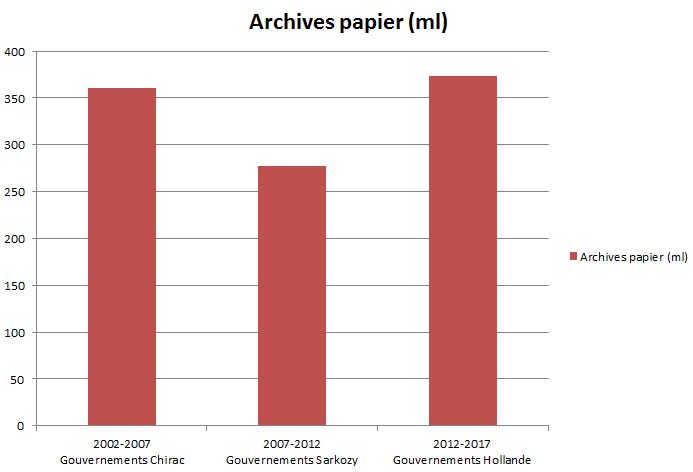
\includegraphics[width=\textwidth]{illustrations/figure7.1.png}
		\caption{Diagramme de l’évolution des volumes d’archives papiers collectés}
		\label{figure7.1}
	\end{minipage}
	\hfill %Met un espace entre les deux images.
	\begin{minipage}[b]{0.45\textwidth}
		\centering
		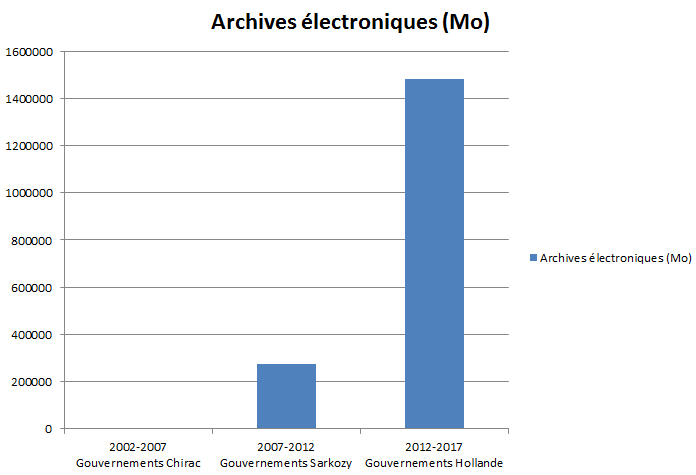
\includegraphics[width=\textwidth]{illustrations/figure7.2.png} 
		\caption{Diagramme de l’évolution des volumes d’archives  électroniques collectés}
		\label{figure7.2}
	\end{minipage}
	\caption{Comparaison de l'évolution des volumes d'archives papiers et électroniques collectés\protect\footnotemark}
	\label{fig:sidebyside1}
\end{figure}
\footnotetext{\textit{Présentation \gls{Archifiltre}}, modèle 2019}

Répondant au programme Entrepreneur d'Intérêt Général\footnote{\enquote{Les Entrepreneur(e)s d’intérêt général (co)pilotent le lancement et l'accélération de services numériques conçus selon l'approche beta.gouv.fr en soutien aux politiques publiques.} (\cite{noauthor_entrepreneur_nodate})} (EIG), le projet \gls{Archifiltre} est alors proposé par Patrice Loriot,  chef du pôle gestion des connaissances (bureau des archives et de la documentation), adjoint au sous-directeur des services généraux et de l'immobilier, et Anne Lambert, cheffe du bureau des archives des Ministères sociaux puis présenté par Anne Lambert et Chloé Moser, adjointe à la cheffe de bureau des archives. Leur candidature a été retenue notamment pour son potentiel de réutilisation dans les différentes administrations et parce qu’il était destiné à un réseau dynamique : celui particulièrement actif et collaboratif des archivistes. Le projet se monte alors d’abord grâce à la collaboration de deux entrepreneurs d’intérêt général recrutés pour lancer l’outil  et les archivistes du service, originellement spécialisés dans les archives papiers, par le biais de nombreux ateliers pour adapter les concepts de visualisation aux archives numériques. Ce travail fait émerger le but principal d’\gls{Archifiltre} : rendre à l’archiviste la sérénité du traitement papier en lui fournissant un outil lui permettant de visualiser et d’intellectualiser efficacement les arborescences.

\subsection{Mise en place d’Archifiltre et développements}
Les réflexions ont rapidement abouti à une première version disponible dès février 2018. Le but était de pouvoir recueillir au plus vite des retours utilisateurs sur l’outil et ainsi des perspectives d’amélioration. Dès cette première parution, la visualisation des arborescences, dite \enquote{visualisation en stalactites}, s’est imposée comme un élément clé de l’outil. Autour de celle-ci, de nombreuses nouvelles fonctionnalités ont été mises en place comme les zooms ou l'ajout de tags directement sur la visualisation de l’arborescence.


\insererImage{0.3}{illustrations/figure8.png}{Visualisation en stalactites de l'application Archifiltre}{figure8}


Le développement d’un export au format CSV compatible avec l’outil de préparation de \gls{SIP} ReSIP a permis à \gls{Archifiltre} de s’inscrire dans la chaîne de préparation des  versements dans des \gls{SAE} basés sur la solution \gls{VITAM}, en particulier celui des Archives nationales. Le 29 novembre 2018, le premier versement aux Archives nationales est d’ailleurs effectué par les Ministères sociaux ayant utilisé pour la première fois la chaîne de traitement qui allait devenir commune : l’étude de l’arborescence avec \gls{Archifiltre}, la préparation du \gls{SIP} avec ReSIP et le versement dans ADAMANT basé sur la solution \gls{VITAM}. 


Par ailleurs, la crise sanitaire de 2020 a joué un rôle important dans l'accélération de l'adoption d'\gls{Archifiltre}. En effet, son utilisation s’est accrue notamment car les archives papiers étant inaccessibles en télétravail, le traitement des archives numériques s’est développé. Pendant cette période de télétravail forcé, le choix a été fait de consacrer du temps à la formation et à la documentation sur l’outil, une documentation détaillée a été créée et de nombreuses formations ont été dispensées aux archivistes souhaitant profiter de ce temps forcé en télétravail pour se mettre à l’archivage électronique. L’outil étant en début de chaîne de traitement, il a par ailleurs constitué pour beaucoup un moyen de commencer à appréhender les archives numériques et la transition vers cette nouvelle part du métier d’archiviste. En conséquence de la crise sanitaire, une très nette réduction de la production papier a été observée, tandis que la production  électronique continue d’augmenter, profitant également au développement d’\gls{Archifiltre}.


En 2022, \gls{Archifiltre} élargit son champ d'action avec le projet Archifiltre-Mails, un outil de visualisation et de tri des messageries, financé par un appel à projet. Cet élargissement illustre l'impact significatif d'Archifiltre dans la gestion et l’adoption de méthodes pour le traitement des archives numériques en France. Ce projet devient prioritaire et le reste jusqu’en janvier 2024 où le choix est fait de le mettre en pause au profit de la première application d’\gls{Archifiltre}, renommée \enquote{Archifiltre-Docs\footnote{En juillet 2024, l’équipe a fait le choix de renommer Archifiltre-Docs en \gls{Archifiltre} par souci de clarté et pour s’adapter à l’usage.}}.


Enfin, \gls{Archifiltre}, grâce à sa relative simplicité et son utilité pour la compréhension d’arborescences, a vu son audience grandir au-delà des archivistes pour s’élargir à des agents de services numériques, aux services producteurs et finalement au grand public\footnote{Un schéma récapitulatif des étapes du développement d'Archifiltre est disponible en annexe \ref{annexe1}.}.

	
	\part{La gestion des données de la chaîne de traitement des archives des ministères}
	
	
\chapter{Le SEDA et son fonctionnement}

Une chaîne de traitement se met donc en place au sein des services d’archives des ministères. Au cœur de cette chaîne se trouvent les données qui constituent la source de l’information de l’archive numérique\footnote{Pour en savoir plus sur les données au coeur du fichier numérique, voir \cite[pp.253-256]{nguyen_chapitre_2020}.}. Ces dernières peuvent prendre de nombreuses formes différentes. Afin de garantir leur intégrité et leur pérennité, un standard est créé : le Standard d’échange des données archivistiques ou \gls{SEDA} dont les lieux d'action sont résumés par le schéma suivant\footcite{nichele_formation_2022} : 

\insererImage{0.4}{illustrations/figure9.png}{Schéma des lieux d’actions du \gls{SEDA} au sein de la chaîne d’archivage électronique}{figure9}


\subsection{Historique du SEDA : construction et évolution}
Le Standard d'Échange de Données pour l'Archivage (\gls{SEDA}) a vu le jour afin de répondre au besoin d’un cadre normatif pour les échanges de données entre services publics d’archives et leurs partenaires. Son élaboration a débuté en 2005 par une collaboration entre la direction des archives de France (DAF) et l'ancienne Agence pour le Développement de l'Administration Électronique (ADAE), dans le cadre de l'action 103 du programme ADELE (Administration électronique). Cette collaboration s’est poursuivie par des échanges suite à un appel à commentaires clôturé le 23 décembre 2005, suivi d'ateliers entre décembre 2005 et janvier 2006\footcite{cines_oais_2019}. Cela a permis de fortement généraliser le début de standard qu’était alors le \gls{SEDA} en s'appuyant non seulement sur ces échanges mais également sur des normes existantes comme le langage \gls{XML} (\textit{eXtensible Markup Language}), la norme ISO 14721 (modèle \gls{OAIS}), la \gls{DTD} \gls{EAD} (Description archivistique encodée) et la norme NF Z 42-013 sur l’archivage électronique\footcite[p.63]{gueit-montchal_chapitre_2020}.  


Le \gls{SEDA} passe ensuite de standard à norme avec sa transposition à la norme NF Z44 0-22 \enquote{Modélisation des échanges de données pour l’archivage} (MEDONA) en janvier 2014. Ce passage à la norme nationale puis internationale, avec la normalisation à l'ISO qui a abouti à la norme ISO 20614 \enquote{ Protocole d'échange de données pour l'interopérabilité et la préservation} (DEPIP), l’a fait évoluer : le standard qui était d’abord spécifique aux archives publiques s’est élargi pour pouvoir être appliqué plus largement\footcite{b2c_dstandard_2018}. C’est à partir des élargissements donnés au \gls{SEDA} à travers ces processus de normalisation auxquels s'ajoutent notamment les réflexions de l'équipe du Programme \gls{VITAM} que s’élabore le \gls{SEDA} 2\footcite{jacobson_standard_2014}. Il prend en compte les modifications adoptées par le \gls{SEDA} pour son passage à la norme MEDONA et les comités de pilotage du \gls{SEDA} 2 le spécialisent de nouveau pour le cas des archives publiques. Ce travail aboutit à la publication de sa version 2.0 en décembre 2015.


\subsection{Organisation globale du SEDA : but}

Le \gls{SEDA} repose sur plusieurs schémas \gls{XSD}, consultables sur le site \href{https://francearchives.gouv.fr/seda/2.2/documentation/html/seda-2.2-main.html }{FranceArchives}, et vise à faciliter l’interopérabilité entre les systèmes d’information des services d’archives et ceux de leurs partenaires. Il modélise sept transactions spécifiques liées à l'archivage de documents ou données électroniques entre le service versant, le service d’archives et des tierces entités : 
\begin{itemize}
	\item le transfert, 
	\item la demande de transfert, 
	\item l’élimination, 
	\item la communication, 
	\item la demande d’autorisation, 
	\item la modification,
	\item la restitution. 
\end{itemize}


Ces transactions impliquent six acteurs principaux : 
\begin{itemize}
	\item le service producteur, 
	\item le service versant, 
	\item le service d'archives, 
	\item le service de contrôle, 
	\item le demandeur d'archives, 
	\item l'opérateur de versement, depuis la version 2.0\footcite[pp.34-35]{dieng_qualite_2020}.
\end{itemize}


Les formats, structures et contenus informationnels échangés sont clairement définis dans le standard. Par ailleurs, le \gls{SEDA} bénéficie d'une structure modulaire permettant une adaptation aux différents besoins et est mis à jour régulièrement depuis la reprise des travaux en 2020 afin d’intégrer les besoins exprimés par les membres du comité de pilotage\footcite{noauthor_standard_2024}. La dernière version du \gls{SEDA}, la 2.3, est d’ailleurs parue fin juillet 2024, alors que ce travail est en cours de rédaction, et la documentation associée devrait être publiée d’ici la fin de l’année 2024. 

\subsection{Description technique de l’organisation du SEDA 2.2}

Cette organisation conceptuelle globale est concrètement mise en œuvre dans le schéma \gls{XML} au travers de ses balises et de leur organisation. En effet, les balises du \gls{SEDA} sont organisées en 4 types de métadonnées : 
\begin{itemize}
	\item les \textbf{métadonnées techniques} qui décrivent les aspects techniques des documents archivés, comme le format de fichier, la taille, le logiciel utilisé pour créer ou modifier les documents, les spécifications de numérisation et les informations sur l'intégrité des données (par exemple, les sommes de contrôle ou les signatures numériques). Ces métadonnées permettent de garantir que les documents peuvent être correctement lus et interprétés sur le long terme, indépendamment des évolutions technologiques.
	\item les \textbf{métadonnées de gestion} qui sont employées pour administrer et surveiller les documents au cours de leur cycle de vie archivistique. Elles incluent des informations sur les règles de conservation, les droits d'accès, les politiques de gestion des archives, les actions effectuées sur les documents (comme les transferts ou les éliminations) et les responsables des différentes actions. Ces métadonnées garantissent la bonne gestion et la traçabilité des documents archivés.
	\item les \textbf{métadonnées de transport} qui sont liées au transfert physique ou électronique des documents entre différents systèmes ou entités. Elles contiennent des informations sur l'expéditeur, le destinataire, le format de transfert, la date et l'heure de l'envoi, ainsi que des accusés de réception. Ces métadonnées assurent l'intégrité et la sécurité des documents lors de leur transfert et facilitent le suivi des échanges.
	\item les \textbf{métadonnées de description} qui contiennent des informations contextuelles et descriptives sur les documents archivés (titre, auteur, date de création, etc.) dont l’organisation est inspirée de la norme \gls{ISAD(G)} (\textit{International Standard Archival Description - General}) et de sa déclinaison technique l’\gls{EAD}. Ces métadonnées permettent de comprendre le contenu et la provenance des documents, facilitant ainsi leur recherche et leur identification dans le système d'archivage.
\end{itemize}


Par ailleurs, en plus de ces 4 types de métadonnées, il existe des balises qui décrivent le type de message en fonction de la raison de l’échange de données. Elles sont essentielles pour structurer et gérer les différents types de messages échangés dans le cadre du \gls{SEDA} et ainsi garantir une communication standardisée et efficace entre les divers acteurs du processus d'archivage. Les balises sont les suivantes : 
\begin{itemize}
	\item <BusinessMessageType> (message de transfert), balise utilisée pour initier le transfert de documents ou de données d'un service versant vers un service d'archives.
	\item <BusinessMessageReplyType> (message de demande de transfert), balise utilisée pour répondre à une demande de transfert, indiquant l'acceptation ou le rejet de la demande initiale.
	\item <BusinessRequestMessageType> (message d'élimination), balise utilisée pour demander l'autorisation de détruire des documents archivés.
	\item <BusinessRequestMessageType> (message de communication), balise utilisée pour demander l'accès à des documents archivés.
	\item <BusinessRequestMessageType> (message de demande d’autorisation), balise utilisée pour demander l'autorisation de réaliser une action spécifique sur des documents archivés.
	\item <BusinessMessageType> (message de modification), balise utilisée pour notifier une modification sur des documents archivés ou sur leurs métadonnées.
	\item <BusinessRequestMessageType> (message de restitution), balise utilisée pour demander la restitution de documents archivés à leur service d'origine ou à une autre entité.
	\item <Acknowledgement> (message d'accusé de réception), balise utilisée pour accuser réception d'un message, confirmant qu'il a été reçu et traité.
\end{itemize}


Dans ce cadre, il existe 4 balises communes à tous les types de messages : <Comment>, <Date>, <Message Identifier> et <Signature> dont seules <Date> et <MessageIdentifier> sont obligatoires et sont toujours positionnées en début de \textit{\gls{manifest}}\footcite[pp.43-45]{siaf_dictionnaire_2022}.


Enfin, les différents types de métadonnées sont liés entre eux par des systèmes de références (id) qui permettent de garder associées les différentes métadonnées qui renvoient au même fichier (binaire) archivé. 

\subsection{Le champ d’action de l’utilisateur sur le SEDA dans le cadre de la chaîne de traitement définie}
Dans le cadre de la chaîne de traitement définie dans la première partie de ce travail, l’utilisateur manipule des données qui se présentent soit sous la forme de documents soit sous la forme de métadonnées associées soit sous la forme de base de données. Ces données sont ordonnées à l’aide du schéma \gls{XML} \gls{SEDA} au cours de la chaîne de traitement. Pour l’utilisateur, il n’est pas nécessaire de comprendre l’entièreté des balises exactes enrichies et la logique pleine du \gls{SEDA} derrière l’interface des outils, bien qu’il reste aujourd’hui important d’en maîtriser les bases logiques, les outils n’effaçant pas totalement la présence de ce standard d’échange.


Au sein d’\gls{Archifiltre}, seules les sous-balises de la balise <ArchiveUnit> sont enrichies. Chaque document intellectuel est une \enquote{\textit{Archive Unit}} ou \enquote{\gls{unité d’archives}} (UA). Au sein de cette balise, il est donc possible d’ajouter toutes les informations spécifiques à cette entité intellectuelle. \gls{Archifiltre} se concentre sur l’enrichissement de la balise <content>, définie dans le dictionnaire du \gls{SEDA} 2.2 comme un \enquote{bloc de « Contenu » de l’\gls{unité d’archives} qui contient toutes ses métadonnées de description}\footcite[p.13]{siaf_dictionnaire_2022}. Au sein de l’outil ReSIP, cette balise est nommée \enquote{descriptif}. Archifiltre permet dans son \enquote{export Resip} le chargement de l’arborescence ainsi que l’enrichissement automatique des sous-balises de <content> dans cet outil. 


Au sein de ReSIP, il est par ailleurs possible d’enrichir une autre sous-balise de la balise <ArchiveUnit>, <management> définie dans le dictionnaire du SEDA 2.2 comme \enquote{Métadonnées de gestion associées à une \gls{unité d’archives}}\footcite[p.13]{siaf_dictionnaire_2022}. L’ensemble des sous-balises de <content> et <management> est listé en annexe\footnote{Cf. Annexes \ref{annexeb} et \ref{annexec}} avec leur traduction française dans ReSIP et  leur définition. Dans l’outil ReSIP, il est également possible de remplir les métadonnées communément appelées \enquote{métadonnées d’en-tête}. Ces métadonnées sont liées au type de message et incluent notamment les quatres balises communes à tous les types de messages précédemment détaillées. Ces métadonnées sont complétées dans l’onglet \enquote{Métadonnées globales} de l’onglet \enquote{Editer les informations d’export}. Les métadonnées de transports sont quant à elles en partie renseignées et modifiables dans ce même onglet au deuxième volet, accompagnées de certaines métadonnées associées au type de message et des métadonnées globales de gestion qui s’appliquent à l’ensemble du versement et non pas à une archive spécifique.

\insererImage{0.35}{illustrations/figure10.png}{Onglet \enquote{Editer les informations d’export} de ReSIP}{figure10}


Enfin, au-delà des nombreuses informations que le \gls{SEDA} permet d’organiser et de pérenniser dans ses différentes balises, le schéma permet également l’extension à des balises d’autres schémas \gls{XML} comme par exemple l’\gls{EAD}, le \textit{Dublin Core} ou encore METS (\textit{Metadata Encoding and Transmission Standard}) afin d’assurer la prise en compte totale de tous ses usages. Néanmoins, cette utilisation est rendu impossible par les outils de la chaîne de traitement et par les différentes versions du \gls{SAE} \gls{VITAM}, notamment celui des Archives nationales, dans lesquels ce type d’extensions sont bloquées. La volonté d’exhaustivité du \gls{SEDA} est également limitée par certaines règles définies dans ces outils qui le contraignent davantage. Lorsque l’on verse dans ADAMANT, le \gls{SAE} des Archives nationales, il n’est par exemple pas accepté d’avoir un \textit{\gls{manifest}} dans lequel la balise <CustodialHistory> (Historique de conservation) aurait plus d’une seule sous-balise <CustodialHistoryItem>. Ainsi, malgré son apparente adaptabilité, la pratique du \gls{SEDA} peut s’avérer plus limitante suivant les choix des structures qui l’ont implémenté. 


Ainsi, le \gls{SEDA} permet d’assurer la pérennité et l’intégrité des métadonnées lors de leurs échanges au cours de la chaîne de traitement des archives. Néanmoins, son utilisation reste compliquée à la fois par les outils de la chaîne de traitement qui le limitent et par la difficulté que sa prise en main représente pour un grand nombre d’archivistes aujourd’hui. 
\chapter{Le cas de l’archivage des systèmes d’information}

\subsection{Les nouveaux objets électroniques à archiver}
A l’aide de la chaîne de traitement telle que décrite précédemment, une méthodologie pour l’archivage des fichiers bureautiques et audiovisuels a pu être établie. Grâce à elle, les données de ces documents sont facilement converties en \gls{SEDA} dans des \gls{SIP}. Néanmoins, bien que représentant la majorité des informations électroniques à archiver, les fichiers bureautiques et audiovisuels n’en constituent pas la totalité. Certaines typologies plus complexes demandent une attention particulière et surtout une adaptation des méthodes et des outils\footcite[p.95]{dangio-barros_archivage_2013}. En effet, aujourd'hui des objets numériques complexes comme les mails, au format .pst le plus souvent dans l’administration française, attirent l’attention des spécialistes et des solutions sont encore en train d’être réfléchies\footnote{Pour en savoir plus, voir :\cite{programme_vitam_larchivage_2013}}.


Depuis le programme \textit{Action publique 2022} (AP2022) porté par le Premier ministre en 2017 et visant à la dématérialisation de l’ensemble des processus administratifs, les projets de systèmes d’information nationaux\footnote{D’après le décret n° 2014-879 du 1er août 2014 relatif au système d'information et de communication de l'Etat, un \enquote{système d'information et de communication de l'Etat est composé de l'ensemble des infrastructures et services logiciels informatiques permettant de collecter, traiter, transmettre et stocker les données sous forme numérique qui concourent aux missions des services de l'Etat.} <\href{https://www.legifrance.gouv.fr/loda/id/JORFTEXT000029337021}{https://www.legifrance.gouv.fr/loda/id/JORFTEXT000029337021}>} se sont renforcés et multipliés. Outre le changement de supports et d’acteurs agissant sur ces archives induit par un tel bouleversement, cela a également renforcé le besoin de maîtriser les données des systèmes d’information afin de les archiver efficacement\footcite{banat-berger_note_2023}. Or, les données que ces systèmes contiennent peuvent être multiples, sous forme de documents déposés, de bases de données ou autre. 


Dans une \textit{Note sur l'archivage centralisé des données, documents numériques et métadonnées issus des systèmes d'information nationaux de l'État} datant du 03 août 2023, Françoise Banat-Berger, cheffe de service du Service interministériel des archives de France (SIAF), affirme la responsabilité de la Mission des archives de France et des services d’archives ministériels dans le \enquote{traitement et le transfert} des \enquote{données, documents et métadonnées} des systèmes d’information nationaux \enquote{vers les Archives nationales, en vue de leur archivage définitif}. Pour faire face à cette mission, le Ministère de l’Agriculture a notamment créé une grille d’étude des systèmes d’information appelée \enquote{étude CYCLAD}\footnote{Voir la grille d'étude CYCLAD en annexe \ref{annexed}} (Cycle de conservation légal et d'archivage des données). Cette grille est également utilisée par les Ministères sociaux et permet aux archivistes de faire un état des lieux des données présentes dans les systèmes d’information, de leur importance historique et juridique et de leurs durées de conservation afin de définir en amont une stratégie efficace d’archivage. 


Par ailleurs, il faut noter que la définition concrète de cet enjeu dans l’objectif 8.2 \enquote{Archiver au niveau central les données des services déconcentrés de l’Etat issues d’applications développées et maintenues au niveau central} du \textit{Cadre commun stratégique de modernisation des archives} pour la période 2020-2024\footcite{noauthor_cadre_nodate} appuie également l’importance que la maîtrise de l’archivage des systèmes d’information va continuer de prendre dans les années futures.

\subsection{La naissance d’un besoin au travers de l’expérience des Ministères sociaux}
\label{part2.chap2.2}

Au bureau des archives des Ministères sociaux, porteurs de l’outil \gls{Archifiltre}, la problématique de l’archivage des systèmes d’information (\gls{SI}) s’est imposée d'elle-même au fur et à mesure des cas d’usage. C’est en 2019 que le service a traité son premier cas d’archivage de système d’information avec le \gls{SI} Papyrus gérant l’ensemble des rapports de l’Inspection générale des affaires sociales (IGAS). Ce premier cas était peu complexe car il ne comportait qu’une base de données à archiver. 


En revanche, Chloé Moser, adjointe à la cheffe de bureau et \textit{Product owner} d’\gls{Archifiltre}, avait pu suivre, au titre du contrôle scientifique et technique, en 2019 le décommissionnement d’un \gls{SI} de l’Agence nationale de sécurité sanitaire de l'alimentation, de l'environnement et du travail (ANSES) qui possédait un niveau de complexité supérieur. La volonté était de récupérer les métadonnées du \gls{SI} pour enrichir les documents versés dans le \gls{SAE} de l’ANSES. Pour mener à bien cet objectif, c’est le prestataire Mintika qui a effectué les exports. Dès lors, au sein du service est née une réflexion sur le manque d’autonomie qu’une telle solution crée. Il a semblé alors nécessaire de trouver un moyen pour pouvoir effectuer les exports sans avoir besoin de faire appel à un prestataire pour chaque \gls{SI}.


En 2021, le cas du système d’information CONTIX+ marque un tournant dans les réflexions et confirme le besoin d’un outil qui permette l’archivage des \gls{SI} complexes. CONTIX+ est un \gls{SI} de la Direction des affaires juridiques (DAJ) des Ministères sociaux qui permet le suivi des contentieux. Son décommissionnement a été décidé afin de le remplacer à la fois par un espace \textit{Sharepoint} et par la plateforme télérecours du Conseil d’Etat. La complexité de son archivage réside dans le fait qu’il ne s’agisse pas simplement d’une base de données mais à la fois de documents et de métadonnées associées. Ainsi, lors de l’export du \gls{SI} pour archivage nous nous retrouvons avec une arborescence de documents d’un côté et un fichier CSV de l’autre. Ce fichier CSV est constitué d’autant de colonnes qu’il y a de catégories de métadonnées à extraire de ce \gls{SI} et autant de lignes qu’il y a de documents extraits. Ainsi, les documents ne sont associés qu’aux métadonnées minimum classiquement attachées à des documents comme la date de création, le titre ou le format et il est nécessaire de trouver la ligne du CSV qui leur correspond afin de connaître des informations supplémentaires entrées dans le \gls{SI} et les concernant. L’archivage de ce \gls{SI} s’avérant être un bon exemple des problématiques auxquelles les archivistes vont être de plus en plus confrontés dans un futur relativement proche, le service des archives des Ministères sociaux a fait appel au prestataire Olkoa grâce au financement obtenu par une prestation DIAMAN\footcite{noauthor_appel_2024} (Dispositif d'accompagnement des missions pour l'archivage numérique). Avec leur aide, un plan d’archivage de CONTIX+ a pu être mis en place et les premières réflexions sur le moyen de faire évoluer l’outil Archifiltre afin de rendre l’archivage des \gls{SI} moins complexe ont été menées. Le diagramme suivant présente ce plan d'archivage. Il est constitué de trois étapes : l'analyse du contenu de la base de données et des fichiers, la préparation du versement et le versement.

\clearpage

\insererImage{0.8}{illustrations/figure11.png}{Diagramme de la méthodologie de versement d’une application métier à décommissionner réalisé par Olkoa.}{figure11}


En conclusion de cette étude ressort globalement l’idée de créer une nouvelle fonctionnalité qui s'insèrerait dans la deuxième étape du processus décrit ci-dessus. Elle permettrait d’importer le CSV contenant des métadonnées supplémentaires extraites de \gls{SI} comme décrit ci-dessus dans \gls{Archifiltre}. Après l’import de l’arborescence extraite du \gls{SI}, tel qu’il se fait classiquement dans \gls{Archifiltre}, ce CSV pourrait alors être importé . Chaque ligne de ce CSV serait ensuite associée au document à laquelle elle se réfère. Ainsi, l’export \gls{Archifiltre} destiné à être importé dans ReSIP et à être versé à terme dans le \gls{SAE} \gls{VITAM}, serait enrichi afin d’y ajouter les métadonnées supplémentaires associées directement aux bons documents. Cet export enrichi vers ReSIP permettrait alors d’alimenter automatiquement les métadonnées de description de la balise <Content> et les métadonnées de gestion de la balise <management> pour chaque document, c’est à dire pour chaque \gls{unité d’archives} (ou <ArchiveUnit>).

\clearpage

\insererImage{0.4}{illustrations/figure12.png}{Description générale du besoin par Olkoa}{figure12}


Le besoin d’archivage des \gls{SI}, décrit par Olkoa ci-dessus spécifiquement pour être traité par \gls{Archifiltre}, est un besoin dont se sont saisis quelques acteurs comme l’Institut national de la propriété industrielle\footcite[p.10]{disic_mandat_2012} (INPI), le Ministère de la Justice ou encore le Commissariat à l'énergie atomique et aux énergies alternatives (CEA). Néanmoins, leur travail se concentre sur la mise en place d’un archivage en flux automatique à l’aide d’un connecteur. En s’intéressant à cette problématique, \gls{Archifiltre} cherche à proposer une solution alternative à la mise en place de ces solutions très coûteuses\footcite[p.12]{disic_mandat_2012} pour les services d'archives.


Suivant le but ainsi défini, un premier \gls{POC} (\textit{Proof of concept}) a été produit en septembre 2022.  Celui-ci avait pour but de confirmer rapidement la faisabilité de cette idée à l’équipe en interne et non pas d’être publié. Son utilisation était très limitée et la fonctionnalité avait alors été construite afin d’être testée précisément sur un CSV défini. Elle ne concernait également que l’import de métadonnées supplémentaires sans aborder l’association de ces dernières aux balises \gls{SEDA} adaptées lors de l’export vers ReSIP. Loin d’être abouti, ce premier POC a néanmoins permis de confirmer à l’équipe l’intérêt d’une telle fonctionnalité et lui a donné des premières pistes de réflexions pour établir les bases d’une future fonctionnalité plus développée. 


En conclusion, le besoin de faire évoluer les outils face à la problématique de la complexité des systèmes d’information à archiver se fait de plus en plus présent. L’équipe \gls{Archifiltre} a profité de ses expériences d’archivistes afin de se saisir du problème et de tenter de proposer une solution via son outil. Néanmoins, il est primordial que dans le développement de cette solution, les contraintes de la chaîne de traitement telle que définie dans la première partie de ce travail soient correctement prises en compte. De plus, le standard d’échange \gls{SEDA} constitue à lui seul une complexité inévitable pour l’équipe comme pour l’ensemble des archivistes numériques. Il est donc essentiel de le comprendre et de s’adapter à ses contraintes et à son fonctionnement afin de proposer une solution viable et facilitant l’emploi du \gls{SEDA} pour les archivistes. 



	\part{La mise en place d’une nouvelle fonctionnalité pour Archifiltre}
	
	
\chapter{Fonctionnement de l’équipe Archifiltre}

L’équipe \gls{Archifiltre} décide donc de développer une nouvelle fonctionnalité qui permettrait d’associer les métadonnées supplémentaires aux documents extraits du même système d’information. Pour ce faire, elle met en place une méthodologie lui permettant de s’assurer de la conformité aux attentes des utilisateurs et à l’environnement technique tout au long du développement. Nous la présenterons en détaillant tout d’abord le fonctionnement et les méthodes employées par \gls{Archifiltre} au quotidien. Nous exposerons ensuite les étapes du développement de cette nouvelle fonctionnalité et les moyens utilisés afin que ce travail s’adapte aux besoins utilisateurs comme au cadre technique et normatif définit dans les premières parties de ce mémoire. Enfin, nous aborderons les étapes post-développement à mettre en place afin d'assurer l’adoption de cette fonctionnalité par les utilisateurs. \\


\gls{Archifiltre} fait partie des \textit{startup} d’Etat portées par la Fabrique des Ministères sociaux\footnote{Cf. Introduction (\pageref{Introduction})}. Cette appartenance lui impose une certaine façon de travailler et notamment l’usage de l’\gls{agile} et du mode produit.


\subsection{Le choix de l’agile et de l’approche produit}
\gls{Archifiltre} a en effet adopté un fonctionnement basé sur la méthode \gls{agile} en la modifiant afin de la rendre conforme à l’équipe et ainsi plus facilement adaptable aux besoins utilisateurs. Cette organisation que l’on peut qualifier d’\gls{agile} souple découle de l’adoption du choix du mode produit à la place du mode projet, plus répandu au sein de l’administration française, correspondant à la dichotomie maîtrise d’ouvrage / maîtrise d'œuvre. Des formations à l’\gls{approche produit} sont notamment organisées par la Fabrique des Ministères sociaux\footcite{betagouv_guide_2024}. 


Le principe essentiel de ce changement de paradigme est la volonté de replacer au centre des réflexions et des développements l’utilisateur et ses besoins\footnote{\cite{baheux_mode_2024}. Pour en savoir plus : \cite{sponheim_what_2024}}. En effet, en mode produit un des points d’attention principaux est la réponse aux besoins et la résolution des problèmes rencontrés par les utilisateurs. Le produit est considéré comme une proposition constamment testée par les utilisateurs. Le recueil du besoin et des retours utilisateurs prend donc une place importante dans le travail effectué.


Par ailleurs, la différence entre ces deux méthodes de conduite de projet réside également dans l’organisation du travail\footcite[p.21]{betagouv_guide_2024}. En mode projet, la conception est séparée de l’exécution. Un cahier des charges est défini en amont par les équipes métiers. Il détaille et guide l’exécution du projet informatique par les équipes en charge des aspects opérationnels. En mode produit, l’équipe est pluridisciplinaire. Elle mêle des personnes avec des compétences métiers et des personnes chargées du développement et conçoit, construit et opère le produit en intégrant tout le monde à chaque étape.


Enfin, le mode produit et le mode projet sont chacun généralement liés à une méthode de gestion de projet particulière. Le mode projet fonctionne en cycle en V et suit donc une feuille de route précise qui définit le calendrier et le budget alloué à chaque tâche.

\clearpage


\insererImage{0.5}{illustrations/figure13.png}{Schéma explicatif de l’organisation du cycle en V\protect\footnotemark}{figure13}
\footnotetext{\cite[p.12]{betagouv_guide_2024}}


Le mode produit tel qu’il est employé au sein de la Fabrique a quant à lui adopté la méthode \gls{agile}, suivant les principes du \textit{lean startup}\footnote{Cf. Annexe \ref{annexe5}}, afin de pouvoir s’adapter continuellement aux retours utilisateurs. En effet, la méthode \gls{agile} fonctionne en \enquote{\textit{sprint}}, c’est-à-dire en courtes sessions de travail (le plus souvent trois semaines), pour mener à bien une tâche. Au lieu de développer le projet à son maximum dès le début, les équipes vont adopter une méthode itérative et incrémentale\footcite{adam_agile_nodate}. Le but est donc de rendre opérable le plus rapidement possible un \gls{MVP} (\textit{Minimum Viable Product}), c’est-à-dire le minimum viable du produit souhaité. Les équipes vont ensuite continuer à développer le \gls{MVP} en l’améliorant petit à petit à chaque nouvelle version sortie en fonction des retours utilisateurs ce qui permet de réduire le risque d'échec ou d'erreur que l'on peut rencontrer sur des projets classiques. Cela permet également d'apporter de la valeur à l'utilisateur plus rapidement, comme l'illustre le schéma suivant, ce qui est important pour une \textit{startup} d'Etat qui a besoin de prouver sa valeur en continu pour justifier son existence et soutien auprès des sponsors.

\clearpage

\insererImage{0.3}{illustrations/figure14.png}{Comparatif d’un développement produit avec et sans \gls{MVP} \protect\footnotemark}{figure14}
\footnotetext{\cite[p.27]{betagouv_guide_2024}}


\gls{Archifiltre}, notamment en raison de sa nature de \textit{startup} d’Etat, a donc fait le choix de travailler en équipe resserrée mêlant différents métiers en plaçant au centre de leurs développements les retours utilisateurs selon les principes de l’approche produit. Ils se détachent ainsi de la méthode traditionnellement utilisée au sein de l’administration française, l’approche projet. 


Avant de rentrer dans les détails du développement précis d’une fonctionnalité, il est important de présenter plus en détails l’équipe Archifiltre et sa méthode de travail. 

\subsection{Présentation de l’équipe et de son fonctionnement}
L’équipe est actuellement composée de Chloé Moser, \textins{\gls{Product Owner}} et archiviste, de Samuel Pirès, \textit{\gls{Product Manager}}, de Guillaume Lelasseur, développeur et de deux stagiaires archivistes, Manon Saget-Lethias, chargée de communication, et Mathilde Prades, chargée d’expertise fonctionnelle. Le rôle du \textit{\gls{Product Owner}} correspond à un chef de produit digital en mode \gls{agile} et se rapproche du rôle de chargée d'expertise fonctionnelle. Il est responsable de la définition et de la conception d'un produit selon la méthodologie \gls{agile}\footcite{lesparre_product_2023}. Le \textit{\gls{Product Manager}} est quant à lui défini comme \enquote{responsible for evaluating opportunities and determining what gets built and delivered to customers. We generally describe what needs to get built on the product backlog.}\footnote{Traduction : \enquote{chargé(e) d'évaluer les opportunités et de déterminer ce qui sera construit et livré aux utilisateurs. En général, ce qui doit être construit est décrit dans le \textit{backlog} du produit.} (\cite[pp.42-43]{cagan_inspired_2017})}. Le \textit{backlog} produit est une liste ordonnée de tâches, de fonctionnalités ou d'éléments devant être terminés dans le cadre de la feuille de route\footcite{raeburn_gestion_2024}. Ces deux rôles sont complémentaires au sein de l’équipe, d’autant plus que la \textit{\gls{Product Owner}} porte également le savoir archivistique indispensable au bon développement d’un tel outil. Le développeur quant à lui met en œuvre les spécifications définies par le \textit{\gls{Product Manager}}, la \textit{\gls{Product Owner}} et la chargée d'expertise fonctionnelle et les challenge techniquement. La chargée de communication fait vivre la communauté des utilisateurs notamment au travers d’organisation de challenge comme le \textit{Digital Clean Up Day}\footcite{moser_digital_2024} ou le Marathon du tri organisés en 2024 mais également de la tenue du site internet, de la \textit{newsletter} et des différents réseaux sociaux.


Basé sur la méthode \gls{agile} souple employée par \gls{Archifiltre}, chaque semaine est organisée autour de réunions d’équipe ritualisées. Elle commence par un \textit{weekly}, une réunion durant laquelle un retour est fait sur les tâches que chaque membre de l’équipe s’était fixées la semaine précédente. Les tâches de la semaine à venir sont ensuite définies et inscrites dans le calendrier de la première page du \textit{Notion} dédié. L’équipe utilise en effet l’outil \textit{Notion}\footcite{noauthor_documentation_nodate} dans lequel elle organise son travail et centralise la majeure partie des documents produits. Chaque jour de la semaine suivant le \textit{weekly} comporte un \textit{daily}, réunion courte qui permet de partager le travail effectué par chacun, les tâches que chaque membre pense accomplir d’ici le \textit{daily} du lendemain et les éventuels besoins et problèmes rencontrés par les membres. 

\subsection{Méthode double diamant}
Plus spécifiquement, afin de mener à bien le développement de cette nouvelle fonctionnalité, l’équipe \gls{Archifiltre} s’est basée sur les principes de la méthode double diamant. Définie en 2003 par le \textit{UK Design Council}, la méthode dite du \enquote{double diamant}\footcite{design_council_double_nodate} a été pensée pour aider à l’innovation. Elle se compose de quatre étapes : 
\begin{itemize}
	\item La définition du besoin ou de la problématique.
	\item La formalisation et la définition du projet.
	\item Le test et l’itération des différents concepts.
	\item Le développement du produit.
\end{itemize}
Ainsi, en règle générale, on considère que le premier diamant répond à l’affirmation \enquote{\textit{Make sure you build the right product}}\footnote{Traduction : Assurez-vous de construire le bon produit/la bonne solution.} et le deuxième \enquote{\textit{Make sure you build the product right}}\footnote{Traduction : Assurez-vous de le construire de la bonne façon.}.

\insererImage{0.35}{illustrations/figure15.png}{Schéma explicatif de l’organisation de la méthode double diamant\protect\footnotemark}{figure15}
\footnotetext{\cite{noauthor_innovation_nodate}}


Pour le développement de cette fonctionnalité, l’équipe d’\gls{Archifiltre} s’est basée sur ces concepts en les adaptant spécifiquement à leur projet, se concentrant moins sur le suivi rigoureux du contenu de ces quatre étapes tel qu’il est défini par le \textit{UK Design Council} que sur le principe d’ouverture et de fermeture de cette méthodologie qui impose une certaine rigueur et oblige à passer par une logique d’exploration puis de recadrage systématiquement. Elle pousse ainsi l’équipe à étudier un maximum de cas de figure et à identifier des cas d'usages auxquels elle n’aurait pas pensés sans cela, ce qui est primordial dans le contexte spécifique de notre fonctionnalité afin de s’assurer qu’elle s’adapte correctement aux contraintes techniques et normatives de la chaîne de traitement.


Ainsi, lors de la première étape correspondant à l’ouverture du premier diamant,  nous avons effectué plusieurs brainstormings mais également des entretiens utilisateurs et une étude des produits similaires existants (\textit{\gls{benchmark}}). Afin de cadrer les différentes idées et ainsi refermer ce premier diamant en y faisant le tri, le processus d’utilisation de la nouvelle fonctionnalité a été défini ainsi que la \textit{\gls{story map}}, concept qui sera détaillé ultérieurement, à l’aide de la confirmation recueillie lors de tests utilisateurs. C’est à la fin du premier diamant que l’on fait intervenir le développeur. Avec son aide et ses indications techniques, le deuxième diamant est ouvert notamment au sujet de la définition de l’expérience et de l'interface utilisateur (\gls{UX} et \gls{UI}) car le développeur d’\gls{Archifiltre} a également une compétence d’UX designer. Le processus d’utilisation de l’application confirmé par l’étape précédente est alors transformé en une succession de \textit{\gls{wireframe}s}, maquettes de chaque écran que rencontrera l'utilisateur dans l’utilisation de cette fonctionnalité. Ces \textit{\gls{wireframe}s} sont testés et corrigés au moyen de nouveaux tests utilisateurs avant d’être approuvés. La dernière étape consiste alors à rédiger l’ensemble des spécifications destinées à guider le développeur dans son travail afin qu’il construise ce qui a été testé et défini tout au long de cette méthodologie.

Une attention particulière est donc mise sur le développement de l’\gls{UX} et de l'\gls{UI} qui occupe l’ensemble du travail du deuxième diamant. En effet, la volonté d’\gls{Archifiltre} de proposer une utilisation la plus simple et claire possible est ce qui démarque l’application aujourd’hui parmi les différents outils d’archivage électronique. Ainsi, il est primordial pour l’équipe de conserver cette identité qui a favorisé son adoption par les professionnels de l’information et donc d’y accorder une grande importance dans la construction de cette nouvelle fonctionnalité.


Cet ensemble de méthodes constitue alors le socle sur lequel s’appuient les différents travaux nécessaires au bon développement de notre nouvelle fonctionnalité. Elles mettent au centre des préoccupations la flexibilité et l’adaptabilité afin de correspondre au mieux aux besoins utilisateurs. 
\chapter{Etude large du périmètre de la fonctionnalité}


Selon les principes de travail définis précédemment, l’équipe \gls{Archifiltre} commence donc le développement de la nouvelle fonctionnalité d’import de métadonnées en masse en recueillant le besoin utilisateur afin de donner une direction cohérente au cadrage de son développement. Ce recueil, ainsi que le \textit{\gls{benchmark}} qui le suit, font partie de la première étape de la méthode double diamant employée ici. 


\subsection{Définition du besoin utilisateur}
Après avoir constaté théoriquement le besoin montant via les indications du SIAF ainsi que le besoin au sein des Ministères sociaux, il était important d’en faire une étude plus large afin de donner une direction cohérente au cadrage du développement de cette nouvelle fonctionnalité. Quatre archivistes ont été interrogés : 
\begin{itemize}
	\item Anne Lambert, conservatrice du patrimoine et cheffe du service des archives des Ministères sociaux, 
	\item Thibaut Larrède, archiviste hybride au sein des Ministères sociaux, 
	\item Coline Vialle, archiviste  numérique à la métropole de Brest,
	\item Jérome Rouzaire, élève conservateur du patrimoine en stage aux archives municipales de Nice durant lequel il a pu travailler à l’archivage d’un espace \textit{Sharepoint}. Cette expérience ainsi que sa formation récente comprenant de l’archivage électronique en fait un profil particulièrement précieux pour nous.
\end{itemize} 
Ces entretiens étaient relativement ouverts car leur but était avant tout de mieux connaître l’environnement de travail de chacun et ses potentiels impacts sur l'application de la chaîne de traitement afin d’identifier correctement les cas d’usage que notre fonctionnalité devait couvrir pour être utile à cette diversité de profils. Ils ont mené à des discussions sur le besoin d’une fonctionnalité d’association des données supplémentaires issues des systèmes d’information, aussi appelées données-registre, et des documents extraits des \gls{SI} mais également sur la manière dont ces archivistes gèrent aujourd’hui l’archivage des systèmes d’information et plus largement sur les améliorations souhaitées d’\gls{Archifiltre}. 


A partir des informations recueillies et de leur croisement, nous pouvons identifier quatre besoins principaux : 
\begin{enumerate}
	\item Le besoin de pouvoir associer des données-registres à des documents et les exporter dans un tableur correspondant au \gls{SEDA} de ReSIP.
	\item Le besoin de permettre à l’utilisateur de choisir la balise \gls{SEDA} qui correspond à la colonne de métadonnées importée.
	\item Le besoin de pouvoir exporter ce qu’on a fait dans \gls{Archifiltre} et de le ré-importer sur la même arborescence modifiée.
	\item Le besoin d’avoir la possibilité d’importer un vocabulaire contrôlé et/ou de sauvegarder les tags.
\end{enumerate}
Ces besoins sont ceux qui sont principalement ressortis des entretiens lorsque l’on évoque la possible création d’une fonctionnalité \enquote{d’import de métadonnées} avant de préciser la volonté de l’utiliser spécifiquement pour l’archivage des systèmes d’information. Le fait de rester assez large dans un premier temps lors de l’entretien permet de recueillir les réels besoins des utilisateurs sans les biaiser et ainsi de garantir l’ouverture au maximum du premier diamant dans lequel nous nous situons. Ces entretiens nous ont également permis de recueillir des cas d’usage concrets d’utilisation de cette nouvelle fonctionnalité et donc de confirmer son utilité. Jérôme Rouzaire a ainsi évoqué par exemple le cas d’un système d’information gérant les dossiers de contentieux rencontrés lors de son expérience au sein des archives de la métropole de Nice. Lors de l’archivage, une arborescence de documents était extraite d’un côté et un tableur contenant des métadonnées supplémentaires de l’autre. Chaque ligne pouvait être associée à un document. Il était alors nécessaire d’associer ces métadonnées supplémentaires à chaque document au sein du \gls{SIP}, ce pour quoi notre nouvelle fonctionnalité est pensée.

Enfin, ces entretiens ont également permis d’étudier la méthodologie employée, lorsqu’elle existe, au sein des services afin de réussir à archiver les systèmes d’information. Ainsi, Anne Lambert pour le moment combine manuellement l’export \enquote{ReSIP} d’\gls{Archifiltre}, l’export de métadonnées de ReSIP et le fichier contenant les métadonnées supplémentaires extrait du \gls{SI} afin d’obtenir un fichier où toutes les métadonnées d’un même document se situent sur la même ligne du tableur final et les en-têtes de colonnes correspondent au format accepté par ReSIP, c’est à dire des chemins de balises \gls{SEDA}. Par exemple, pour les métadonnées de titre, le nom de la colonne devra être \enquote{Content.Title}\footnote{cf. Annexe \ref{annexe7}}. 


Enfin, il est à noter que l’archivage des systèmes d'information reste aujourd’hui traité au cas par cas par les services d’archives qui sont encore peu nombreux à se saisir du sujet. Ainsi, le développement de cette fonctionnalité présente la particularité de se proposer de répondre à un besoin tout en créant une méthodologie pour un besoin qui n’est encore que futur pour beaucoup de services d’archives. 

\subsection{\textit{Benchmark}}

En parallèle de l’étude du besoin utilisateur, il est important également d’ouvrir les réflexions en étudiant des fonctionnalités similaires déjà existantes. Cet exercice nous permet alors d’identifier les processus auxquels peuvent être habitués nos utilisateurs et de faire un état de l’art de l’\gls{UX} sur nos sujets d’intérêt afin de s’en inspirer, d’éviter des erreurs et ainsi de favoriser l’adoption de notre fonctionnalité. Pour ce faire, un \textit{\gls{benchmark}} est réalisé après avoir défini les sujets d’étude afin de le cadrer sans pour autant le contraindre. Pour cette fonctionnalité, les sujets d’attention du \textit{\gls{benchmark}} sont les suivants : la liberté et la facilité des processus d’import pour l’utilisateur, les formats d’import acceptés et la gestion des erreurs.


Nous étudions alors dans un premier temps les logiciels utilisés communément au sein des services publics d’archives comme ReSIP, \textit{Microsoft Sharepoint}, Ligéo, As@lae, \textit{Excel} et notamment sa fonctionnalité\textit{Power Query}, \textit{Spark Archives}, \textit{OpenRefine} et Brevo. Nous  proposons ensuite de s’intéresser à des logiciels utilisés plutôt dans des entreprises privées comme ArcGIS et Alfresco. Pour ces deux cas, les solutions proposées sont relativement complexes, notamment avec l’utilisation d’\gls{ETL} (extraction, transformation et chargement) ne permettant pas l’autonomie totale des archivistes. Enfin, afin de suivre la logique d’élargissement du premier diamant, nous nous intéressons à des cas éloignés du monde des archives avec l’exemple des réseaux sociaux et notamment d’Instagram. En effet, cette application permet d’importer une ou plusieurs photographies et de leur associer des métadonnées supplémentaires comme une musique, un lieu ou une description et son fonctionnement intuitif est une inspiration intéressante pour atteindre nos objectifs de clarté et de simplicité. 


Nous tirons de ce \textit{\gls{benchmark}} deux principales inspirations : ReSIP et \textit{Power Query} d’\textit{Excel}, pour la simplicité de leurs processus d’import de données et la facilité essentielle de prise en main par l’utilisateur. Le processus d’import de \textit{Power Query} est particulièrement intéressant et se positionne en inspiration principale pour la définition de celui de notre fonctionnalité. 

\clearpage %Permet de garder l'image après ce paragraphe malgré sa taille.

\insererImage{1}{illustrations/figure16.png}{Fenêtre de vérification suite à l’import de métadonnées dans \textit{Excel} (\textit{Power Query})}{figure16}


Par ailleurs, il ressort de ce \textit{\gls{benchmark}}, et notamment de l’étude des différents réseaux sociaux, l’importance de l’utilisation d’icônes ou de noms de boutons clairs et de la cohérence entre cette nouvelle fonctionnalité et le reste de l’application \gls{Archifiltre} déjà existant. Nous tirons également de cette étude la conscience du besoin de proposer une fonctionnalité qui reste techniquement simple à utiliser pour tous et qui permet aux archivistes d’être autonomes dans leur utilisation. Nous excluons donc par exemple la manipulation d’\gls{XML} ou d’\gls{ETL}.


Pour ce qui est de la partie export des métadonnées associées depuis \gls{Archifiltre} afin de les importer dans ReSIP , nous choisissons à ce stade de nous inspirer principalement de la simplicité d’usage de la solution mise en place par Ligéo en laissant à l’utilisateur la possibilité de choisir la balise \gls{SEDA} correspondant à chaque métadonnée à exporter.

\clearpage %Permet de garder l'image après ce paragraphe malgré sa taille.

\insererImage{1}{illustrations/figure17.png}{Interface de \textit{\gls{mapping}} de Ligéo entre l’intitulé de la colonne et une liste dans \enquote{type de champs}}{figure17}



Ainsi, ce \textit{\gls{benchmark}} nous permet d’élargir nos réflexions et de lister des éléments que nous souhaitons intégrer à notre solution à partir de chaque partie utile des outils étudiés en les adaptant aux besoins utilisateurs identifiés précédemment.

\subsection{\textit{Product Requirements Document} et cadrage de l’existant}

Le \textit{\gls{benchmark}} associé aux entretiens utilisateurs nous a donc permis d’explorer un large panel d’options et de besoins afin d’alimenter nos réflexions. Au sein de l’équipe \gls{Archifiltre}, afin de garder une trace de toutes ces réflexions, tout est consigné dans un document qui est alimenté tout au long du développement de la fonctionnalité et qui permet également de le cadrer : le \textit{Product Requirement Document} (\gls{PRD}) ou document d’exigence produit\footcite{formlabs_comment_nodate}. Ce document dont le squelette vierge est consultable en annexe\footnote{Cf. Annexe \ref{annexee}} est rempli par l’équipe tout au long des réflexions et des avancées. Il permet également de guider l’équipe dans les différentes étapes du développement, imposant une certaine rigueur dans la méthode et dans les réflexions simplement par le fait de devoir le compléter. Le \gls{PRD} de la nouvelle fonctionnalité était le principal livrable technique de notre stage.


Un projet débute donc toujours avec l’écriture du début du \gls{PRD}. Ce début impose une explication du contexte au sein de l’application et de la situation actuelle au commencement du développement. Pour notre fonctionnalité, ces parties sont constituées d’un état des lieux de la preuve de concept (\gls{POC}) présente au sein de l’application mais non fonctionnelle ainsi que d’un résumé des observations fournies par Olkoa dans le cadre de leur prestation pour l’archivage de CONTIX+\footnote{Cf. partie 2, chapitre 5.\ref{part2.chap2.2}.}. 


Les conclusions des entretiens utilisateurs ainsi que celles du \textit{\gls{benchmark}} sont inscrites dans leurs parties respectives à la suite de cet état des lieux. L’équipe \gls{Archifiltre} utilisant Notion, les pages des prises de note de chaque entretien ainsi que celle du \textit{\gls{benchmark}} sont liées à leur partie du \gls{PRD}. Une fois ces conclusions définies, la partie définissant les objectifs du développement organisés dans l’ordre de priorité est complétée. Cette partie se situe au début du \gls{PRD} afin d’être facilement visible et mise en valeur à chaque lecture. Ces objectifs doivent en effet guider ensuite l’ensemble du développement. Pour notre nouvelle fonctionnalité, les objectif sont les suivants : 
\begin{itemize}
	\item \underline{Objectif 1 :} Ajouter en masse de nouvelles métadonnées dans \gls{Archifiltre} et les exporter vers ReSIP pour un versement.
	\item \underline{Objectif 2 :} Pouvoir faire l’archivage d’un \gls{SI} ou d’une partie d’un espace collaboratif.
	\item \underline{Objectif 3 :} Pouvoir importer des tags en masse issus d’une liste de vocabulaire contrôlé.
\end{itemize}
Lorsque le développement sera terminé, c’est l’accomplissement de ces objectifs qui permettra de déterminer son succès de manière qualitative.


Une fois le premier diamant ouvert et les objectifs clairement définis, il faut le refermer en triant parmi toutes les options découvertes pendant ce premier travail. Ce choix permet alors de faire émerger un premier processus d’utilisation de ce qui sera la fonctionnalité développée.
\chapter{Définition du périmètre et du processus de la fonctionnalité}
\subsection{Définition du périmètre}
A partir des échanges autour des conclusions de la partie précédente, il est maintenant nécessaire de définir le périmètre de la fonctionnalité.  Pour ce faire, le \gls{PRD} sur lequel nous avons déjà écrit des conclusions à la fois des entretiens utilisateurs mais également du \textit{\gls{benchmark}} est une ressource précieuse. Afin de s’assurer de la cohérence globale de ce périmètre, l’équipe utilise un tableau blanc Miro\footnote{ \href{https://miro.com/fr/}{https://miro.com/fr/}} afin d’y construire des diagrammes décrivant le processus d’utilisation de cette nouvelle fonctionnalité. Un premier processus est défini à l’échelle macro, il s’agit alors seulement de séparer les grandes étapes du parcours des utilisateurs à savoir : l’import, la visualisation des métadonnées importées dans l’interface \gls{Archifiltre} existante et l’export qui doit permettre d’effectuer un \textit{\gls{mapping}} \gls{SEDA}, c’est-à-dire d’associer les métadonnées aux balises \gls{SEDA} auxquelles elles correspondent. Dans un deuxième temps, nous tentons de détailler cette fois ce processus dans un diagramme qui décompose chaque action faite par l’utilisateur. Afin de s’assurer de la cohérence de ce processus, le diagramme décompose l’ensemble des actions réalisées par l’utilisateur depuis l’import de l’arborescence dans \gls{Archifiltre} jusqu’à l’export ReSIP et non pas seulement le processus de la fonctionnalité. 

\clearpage

\insererImage{0.5}{illustrations/figure18.png}{Diagramme d’utilisation de la fonctionnalité import de métadonnées dans \gls{Archifiltre}\protect\footnotemark}{figure18}
\footnotetext{Zooms en annexes \ref{annexe6} et \ref{annexe6.2}}


L’utilisation de la forme diagramme est intéressante car elle aide à imposer une certaine rigueur dans la réflexion. En effet, sa forme nous oblige à décomposer clairement les étapes et donc à être précis dans sa définition. Par ailleurs, tout au long de ce travail, certaines étapes comme la création de ce diagramme peuvent être réalisées par une personne seule. Néanmoins, des réunions sont ensuite organisées pour le présenter et en discuter avec le reste de l’équipe. Ceci permet non seulement de valider à chaque étape ce que l’on produit afin de s’assurer de conserver une direction cohérente mais cela impose également à la personne qui présente une réflexion sur son travail et l’oblige à être claire et à justifier chacun de ses choix. Enfin, certaines personnes de l’équipe sont parfois un peu éloignées du sujet car elles travaillent sur un autre domaine et leurs remarques s’avèrent souvent précieuses car elles possèdent alors plus de recul et une réflexion neuve. 

Le périmètre (ou \textit{scope}) ainsi défini, il est inscrit dans le \gls{PRD} de la façon suivante, reprenant les étapes réalisées par l’utilisateur : 
\begin{enumerate}
	\item Fournir une méthodologie pour l'ajout en masse de métadonnées (voir téléchargement d'un modèle)
	\item Import d’un fichier .csv de métadonnées (glisser/déposer + parcourir les fichiers)
	\item \textit{Mapping} import : définir une donnée pivot automatique et écrasement possible de données déjà dans \gls{Archifiltre}
		\begin{itemize}
			\item Chemin imposé comme donnée pivot dans un premier temps et on propose à l’utilisateur de choisir la donnée pivot dans une prochaine évolution de la fonctionnalité.
			\item Dans une prochaine évolution, possibilité de choisir quelle colonne de métadonnée déjà présente dans \gls{Archifiltre} est écrasée avec quelle colonne de l’import.
		\end{itemize}
	\item Vérification des métadonnées importées (s'assurer que la jointure s’est correctement réalisée) : validation ou annulation 
		\begin{itemize}
			\item Potentiel message d’erreur si toutes les lignes du CSV ne s’associent pas à un fichier/dossier.
		\end{itemize}
	\item Etude des métadonnées importées par visualisation sur les stalactites 
		\begin{itemize}
			\item Affichage des métadonnées individuellement par fichier  (onglet enrichissement amélioré)	
		\end{itemize}
	\item Modifications unitaires des métadonnées importées sur le modèle de ce qu’\gls{Archifiltre} permet déjà de faire.
	\item Export pour étude : 
		\begin{itemize}
			\item Ajout des métadonnées importées dans les exports CSV et \textit{Excel}.
			\item Ajout d’une colonne \enquote{nouvel [nom\_colonne\_importée]} sur le modèle de ce qui est fait pour le nom, chemin, etc en cas de modification unitaire dans \gls{Archifiltre}.
		\end{itemize}
	\item Export pour versement Export ReSIP (SEDA 2.2)
		\begin{itemize}
		\item \textit{Mapping} \gls{SEDA} d'après ce que sélectionne l'utilisateur (se base sur le dictionnaire des balises \gls{SEDA} 2.2 et/ou sur les noms français des balises dans l’interface ReSIP).
		\item Choix dans deux listes déroulantes : \textit{management} (gestion) et \textit{content} (description)
		\end{itemize}
\end{enumerate}

\subsection{La \textit{user story map}}

Une fois le processus défini dans son ensemble, l’équipe l’organise au sein de ce que l’on appelle une \textit{user \gls{story map}}\footcite{miro_modeuser_nodate} ou \enquote{cartographie des récits utilisateurs} en français. La \textit{\gls{story map}} reprend en fait les principes du \gls{MVP} et permet de décomposer en \enquote{\textit{user stories}}, c'est-à-dire en plusieurs processus d’utilisation, les différentes versions de la fonctionnalité\footcite{kaley_mapping_2021}. Comme nous l’avons expliqué précédemment, l’équipe \gls{Archifiltre} fonctionne en mode produit et propose donc le plus rapidement possible un \gls{MVP} à ses utilisateurs avant d’améliorer cette première version en fonction des retours. La \textit{\gls{story map}} permet alors de mettre à plat toutes les idées et de les organiser dans l’ordre de priorité. Dans la première \textit{user story}, qui décrit le processus utilisateur du \gls{MVP}, on ne conserve donc que ce que l’on juge essentiel. On positionne dans les \textit{user stories} suivantes les améliorations possibles par ordre de priorité en fonction de leur pertinence d’après les retours utilisateurs recueillis.
\insererImage{0.3}{illustrations/figure19.png}{\textit{User \gls{story map}} de la fonctionnalité import de métadonnées\protect\footnotemark}{figure19} 
\footnotetext{Zooms en annexes \ref{annexe8.1} et \ref{annexe8.2}.}


Les étapes, que l’on voit ci-dessus en rose, reprennent les actions effectuées par l’utilisateur telles que définies dans le diagramme. Pour chaque \textit{user story}, organisée en \enquote{\textit{release}}, c’est-à-dire en version de la fonctionnalité, on décrit dans les encarts jaunes précisément ce en quoi consiste chaque étape. Il peut y avoir plusieurs encarts pour une même étape car chacun correspond à une action possible. Par exemple, pour l’étape \enquote{visualiser les métadonnées avant import}, les deux étapes sont le détail des messages d’alerte à afficher pour l’utilisateur et la possibilité de valider ou d’annuler l’import. Dans une \textit{user \gls{story map}}, il est essentiel de se limiter à la description des actions et non des visuels afin de ne pas biaiser les réflexions futures.


Enfin, l’intérêt de la \textit{\gls{story map}} est également de pouvoir la modifier et l’alimenter, notamment pour les user stories qui suivent le \gls{MVP}, \textit{a posteriori} à partir des retours utilisateurs.
 
\subsection{Les tests utilisateurs}

Afin de valider le périmètre et la \textit{user story} du \gls{MVP}, il est nécessaire d’éprouver nos choix auprès des futurs utilisateurs pour s'assurer que notre solution est la plus pertinente. Pour ce faire, des tests utilisateurs sont organisés. Ces tests sont fondamentaux dans l’approche produit, ils sont consciencieusement préparés en amont\footnote{\cite{tanovic_customer_2024} ; \cite{ux-republic_guideline_2019}}. Pour diriger un test utilisateur, des hypothèses sont formulées. On construit ensuite un questionnaire afin de pouvoir vérifier ces hypothèses en prenant garde de ne pas influencer les utilisateurs interrogés. Pour ce faire, les questions doivent rester neutres et ouvertes\footcite{buset_leading_2024}. 


Pour ces tests, des archivistes de quatre services d’archives de ministères ont été interrogés : 
\begin{itemize}
	\item Karim Amara, Emilie Godest et Marie-Pierre Diquelou du Ministère de la transition écologique (MTE), 
	\item Anne Lambert et Thibaut Larrède des Ministères sociaux (MS), 
	\item Anne Bourquard du Ministère de l'Agriculture (MA),
	\item Justine Dilien et Julie Wannecque du Ministère de la Culture (MC).
\end{itemize}
Le questionnaire qui a servi de base à chacun de ces entretiens est le suivant : 
\begin{enumerate}
	\item \textbf{Evaluation du besoin (contexte)}
		\begin{itemize}
			\item Effectuez-vous des versements d’archivage électronique dans un \gls{SAE} ? Lequel ?
			\item Pouvez vous me décrire votre méthode de traitement brièvement ?
			\item Avez-vous déjà eu à archiver un \gls{SI}/espace collaboratif (type \textit{Sharepoint}) ? Si oui, quelle méthode avez-vous utilisée ?
			\item Avez-vous déjà eu besoin d’enrichir en masse les métadonnées de documents ? Si oui, quels types de métadonnées (gestion, description, exemples ?) ? Sous quel format étaient ces métadonnées ?
			\item Connaissez-vous et maîtrisez-vous le \gls{SEDA} ?
			\item Utilisez-vous ReSIP pour les versements ? Avec l’export \gls{Archifiltre} ou directement en glissant l’arborescence à traiter/archiver ?
		\end{itemize}
	\item \textbf{Confrontation à nos hypothèses}
	\begin{itemize}
		\item Si vous aviez un outil qui permettait d’associer en masse des métadonnées à des documents, comment l’imagineriez-vous ?
		\item Qu’est-ce qui serait primordial pour vous pour un tel outil ?
		\item Quel format serait le plus adapté à cet import ?
		\item Après, pour avoir nos réponses si ça n’a pas été évoqué instinctivement :  Identifiez-vous le besoin de :
		\begin{itemize}
			\item Vérifier les données importées
			\item Modifier les données importées
			\item Pouvoir remplacer des données déjà associées aux documents
		\end{itemize}
		\item Dans le cadre de l’utilisation d’un CSV de métadonnées pour débuter un traitement dans ReSIP, comment envisagez vous le passage du CSV de métadonnées importé et associé aux documents vers le format ReSIP qui demande d’avoir placé les métadonnées dans des colonnes ayant pour intitulé les balises \gls{SEDA} adéquates ?
		\item \gls{Archifiltre} fait pour l’instant ce \textit{\gls{mapping}} automatiquement, si celui-ci devait se faire par l’utilisateur, comment imaginez-vous l’interface ?
		\item Seriez-vous plus à l’aise pour faire la correspondance entre le nom de la colonne de métadonnées importée et le nom d’une balise \gls{SEDA} ou avec le nom français (comme le fait ReSIP) ?
	\end{itemize}
\end{enumerate}


Une fois les réponses à ces questions obtenues, sachant bien sûr que le questionnaire est adapté en fonction de la discussion, nous leur présentons les détails du périmètre que nous avons imaginé. Ainsi, nous évitons de biaiser leur réflexion en amont et pouvons recueillir leurs réactions spontanées et comparer ce qu’ils ont imaginé de cette fonctionnalité avec ce que nous avons prévu. Le périmètre présenté est celui détaillé dans la partie 3, chapitre 8.1 (p.\pageref{figure18}). Nous le présentons d’abord d’un point de vue macro, en détaillant seulement les grandes étapes à l’aide du diagramme ci-dessous : 

\insererImage{0.42}{illustrations/figure20.png}{Diagramme macro de la fonctionnalité import de métadonnées}{figure20}


Nous recueillons ainsi des premiers retours notamment sur ce qui peut sembler obscur ou contre-intuitif pour l’utilisateur à ce stade. Nous détaillons ensuite chaque étape en présentant les actions faites par l’utilisateur tout au long du processus. 


Ce déroulé d’entretien nous permet donc de vérifier les hypothèses formulées en amont de ce travail à partir des points qui nous semblent susceptibles de bloquer.  
Le résultat de ces tests est résumé par le tableau suivant : 

\clearpage

\begin{table}[h]
	\begin{tabular}{|p{7cm}|p{2cm}|p{2cm}|p{2cm}|p{2cm}|}
		\hline
		\textbf{Hypothèses} & \textbf{MTE} & \textbf{MS} & \textbf{MA} & \textbf{MC} \\
		\hline
		Il est préférable de permettre de faire le \textit{mapping} vers des balises \gls{SEDA} en anglais ET en français de type ReSIP & Oui & Oui & Oui & Oui \\
		\hline
		L’import de métadonnées est un besoin des archivistes des ministères pour archiver les SI & Oui & Oui & Pas encore mais besoin futur & Oui \\
		\hline
		Besoin de pouvoir écraser des données déjà présentes dans \gls{Archifiltre} & Oui & Oui & Oui & Oui \\
		\hline
		Besoin de visualiser les nouvelles métadonnées importées sur le modèle de ce qu’on a déjà dans \gls{Archifiltre}  & / & Oui & Oui mais à voir comment & Oui \\
		\hline
		Besoin de pouvoir modifier unitairement & / & Oui & Non & Oui \\
		\hline
		Besoin de l’interface de vérification avant la validation de l’import & Oui & Oui & Oui & Oui \\
		\hline
		Importer un format CSV est le mieux & Oui & Oui & Oui & Oui mais format \textit{Excel} serait bien aussi \\
		\hline
	\end{tabular}
	\caption{Tableau des résultats de la vérification des hypothèses lors de tests utilisateurs}
\end{table}

Ces résultats permettent de confirmer notre périmètre. Par ailleurs, ils mettent en lumière le fait que la possibilité de modifier unitairement les métadonnées importées est intéressante mais n’est pas prioritaire. Enfin, au-delà de la vérification de ces hypothèses, un bon test utilisateur permet également de faire émerger des besoins ou des idées auxquelles l’équipe n’a pas forcément pensé. En effet, ces échanges sont avant tout faits pour recueillir les réflexions et les réactions les moins biaisées possible et donc, idéalement, permettre de faire ressortir des potentiels oublis de l’équipe lors de leurs réflexions. Nos tests ont par exemple fait émerger une grande diversité en fonction du service d’archives dans les réflexions concernant l’archivage des systèmes d’information mais également une hétérogénéité entre les archivistes dans leur maîtrise des problématiques liées à l’archivage électronique et notamment du \gls{SEDA}. Nous avons notamment pu confirmer le fait qu’il est important de fournir une traduction française des balises \gls{SEDA} mais également le nom original de ces balises car chacun a sa préférence. 
\\

A l'issue de cette fermeture du premier diamant, le processus utilisateur est validé. C’est à ce moment que le développeur intervient et participe à l’ouverture du deuxième diamant concernant la définition de l’interface utilisateur et les choix techniques au bon développement de la fonctionnalité. 
\chapter{Mise en place de l’interface utilisateur}
\subsection{Transmettre le savoir métier}
L’arrivée du développeur dans les réflexions autour de cette nouvelle fonctionnalité met en lumière le travail indispensable de transmission du savoir métier aux personnes non-archivistes de l’équipe. En effet, il est essentiel pour le profil métier de l’équipe, ici la \textit{\gls{Product Owner}} et archiviste ainsi que la stagiaire chargée d'expertise fonctionnelle, de s’assurer que tout le monde a conscience de la culture métier des utilisateurs de cette fonctionnalité. Néanmoins, en ce qui concerne le périmètre de notre fonctionnalité, transmettre l’ensemble des savoirs nécessaires à la pleine compréhension du besoin n’est pas évident. Il a fallu présenter à l’aide d’un exemple la chaîne de traitement détaillée en partie 1 de ce mémoire ainsi que le fonctionnement global de ses outils. Il est également indispensable de transmettre quelques notions d’archivistique et notamment d’expliquer qu’\gls{Archifiltre} ne travaille pas sur les originaux mais sur une image des fichiers afin de garantir l’intégrité des archives. En effet, pour des non-archivistes, ce fait qui empêche par exemple le renommage possible dans \gls{Archifiltre} de s’appliquer sur les originaux, est un point de frustration et d’incompréhension qu’il est nécessaire d’expliquer. Il est également indispensable de transmettre le vocabulaire archivistique mais aussi les notions de \gls{SIP} et de \gls{SAE} relativement complexes à appréhender. Cette étape est d’autant plus importante que le développeur d’\gls{Archifiltre} est qualifié en \textit{UX design} et prend donc part à la définition de l’interface utilisateur. 


Par ailleurs, la plus grande difficulté de transmission, y compris avec quelqu’un de techniquement très qualifié, reste principalement le \gls{SEDA}. Ceci peut notamment s’expliquer par le fait qu’il réponde à des problématiques très précises d’archivistique, parfois même trop spécifiques pour la plupart des archivistes. Nous pouvons également noter que la documentation du \gls{SEDA} reste relativement difficile d’accès et pauvre\footnote{Une nouvelle documentation est néanmoins en cours de préparation et devrait être accessible en décembre 2024.}. Une partie est disponible sur FranceArchives mais se trouve majoritairement sur Github\footcite{noauthor_culturecommunicationseda_2024}, ce qui rend son accès complexe pour un certain nombre d’archivistes. Par ailleurs, le dictionnaire du \gls{SEDA} 2.2\footcite{siaf_dictionnaire_2022}, document selon moi le plus utile pour appréhender le \gls{SEDA} et la logique de son schéma, est construit de telle manière qu’il est difficile de comprendre la hiérarchie concrète des balises et la forme que prend finalement un \textit{\gls{manifest}}. Afin de pallier ces difficultés, nous avons construit un double tableau en nous limitant aux balises pouvant être enrichies pour chaque unité d’archive avec les informations extraites d’un système d’information c’est-à-dire l’ensemble des balises de la balise <content>, métadonnées de description, et de la balise <management>, métadonnées de gestion, pour chaque unité d’archive (<archiveunit>). Le double tableau produit retranscrit les niveaux de hiérarchie des balises et leur associe une traduction française, leur niveau de répétabilité et d’obligation, leur type, leur définition ainsi que des informations particulières à certaines balises comme la liste de termes lorsqu’il s’agit de balises qui n’acceptent qu’une liste de termes définis. Ce document est particulièrement important car il servira ensuite d’appui au développeur pour construire la partie \textit{\gls{mapping}} \gls{SEDA} de la fonctionnalité. Il est consultable en annexes \ref{annexeb} et \ref{annexec}. 


\subsection{Définition des \textit{wireframes} et évolution d’après les retours utilisateurs}

A partir de toutes ces informations et des retours des différents échanges avec les utilisateurs effectués jusque là, le travail de la définition des \textit{\gls{wireframe}s} commence. La première étape consiste à effectuer un \textit{\gls{benchmark}} des interfaces notamment proposées sur le site \textit{Mobbin}\footnote{\href{https://mobbin.com/}{https://mobbin.com/}} et des produits étudiés dans le premier \textit{\gls{benchmark}} mais en l’élargissant à une réflexion uniquement orientée sur l’interface utilisateur (\gls{UI}). Ce \textit{\gls{benchmark}} nous mène à la création des premiers \textit{\gls{wireframe}s} des différents écrans du processus. 


Un \textit{\gls{wireframe}}, ou maquette fonctionnelle, est un schéma qui permet de définir les zones et les différents composants de chaque fenêtre de l’interface utilisateur de notre fonctionnalité. Pour les construire, nous utilisons l’outil \textit{Balsamiq}\footnote{ \href{https://balsamiq.com/}{https://balsamiq.com/}} qui imite le papier et le crayon, fonction importante pour la définition de \textit{\gls{wireframe}s} car le design graphique doit rester absent de cette étape afin de concentrer les réflexions sur l’essentiel. Cet outil permet également de simuler des interactions et de naviguer entre les \textit{\gls{wireframe}}, recréant ainsi le parcours conçu à l'étape précédente. Cette fonctionnalité facilite les tests utilisateurs car elle met en place des conditions un minimum réelles aidant ainsi les utilisateurs à se projeter. En effet, un des points d’attention lorsque l’interface utilisateur est testée est de noter où l’utilisateur clique instinctivement et ce qu’il comprend de l’interface. 


Dans notre cas, il était nécessaire de définir des \textit{\gls{wireframe}s} pour huit étapes du processus : 
\begin{itemize}
	\item La fenêtre d’\gls{Archifiltre} actuelle avec un bouton d’import de métadonnées, 
	\item Une fenêtre de messages de rappel des contraintes à respecter pour l’import,
	\item Une fenêtre d’import du CSV de métadonnées, 
	\item Une fenêtre de sélection de la clé de jointure,  
	\item Une fenêtre qui permet de choisir d’importer ou non chaque métadonnée, 
	\item Une fenêtre de vérification afin de s’assurer de la bonne jointure des données, 
	\item Un nouvel onglet de visualisation tableur des métadonnées importées,  
	\item Une fenêtre qui permet de faire le \textit{\gls{mapping}} avec les balises \gls{SEDA}. 
\end{itemize}
Pour chacun de ces \textit{\gls{wireframe}s}, l’équipe a produit une version puis a fait passer un test utilisateur qui a permis de faire évoluer ces versions. Un autre test a ensuite permis de mettre à l’épreuve les nouvelles versions et de les faire évoluer de nouveau. Cette méthode a été effectuée pour cinq tests utilisateurs jusqu’à obtenir une version répondant à la majorité des blocages rencontrés par les différents utilisateurs. Ainsi, un grand nombre de \textit{\gls{wireframe}s} ont été produits pour aboutir à celles définissant les huit étapes susmentionnées. 


Au cours de ces évolutions, la fenêtre permettant de choisir la colonne de métadonnées du CSV importé correspondant au chemin, jointure imposée pour ce \gls{MVP}, a disparu. Elle est remplacée par l’exigence d’importer un CSV dont la première colonne contient le chemin des fichiers. Cette exigence est indiquée dans la fenêtre de message de rappel qui se présente comme une liste à cocher de quelques consignes à respecter comme le format CSV ou le format des dates importées. Soumettre l’import au fait de cocher les cases est le choix qui a été fait à l’issue de l’ensemble de tests utilisateurs afin de garantir le fait que ces indications soient prises en compte. 

\clearpage

\begin{figure}[h]
	\centering
	\begin{minipage}[b]{0.45\textwidth} %Crée une sous-structure dans le document qui prend ici 45% de la largeur totale de la ligne.
		\centering
		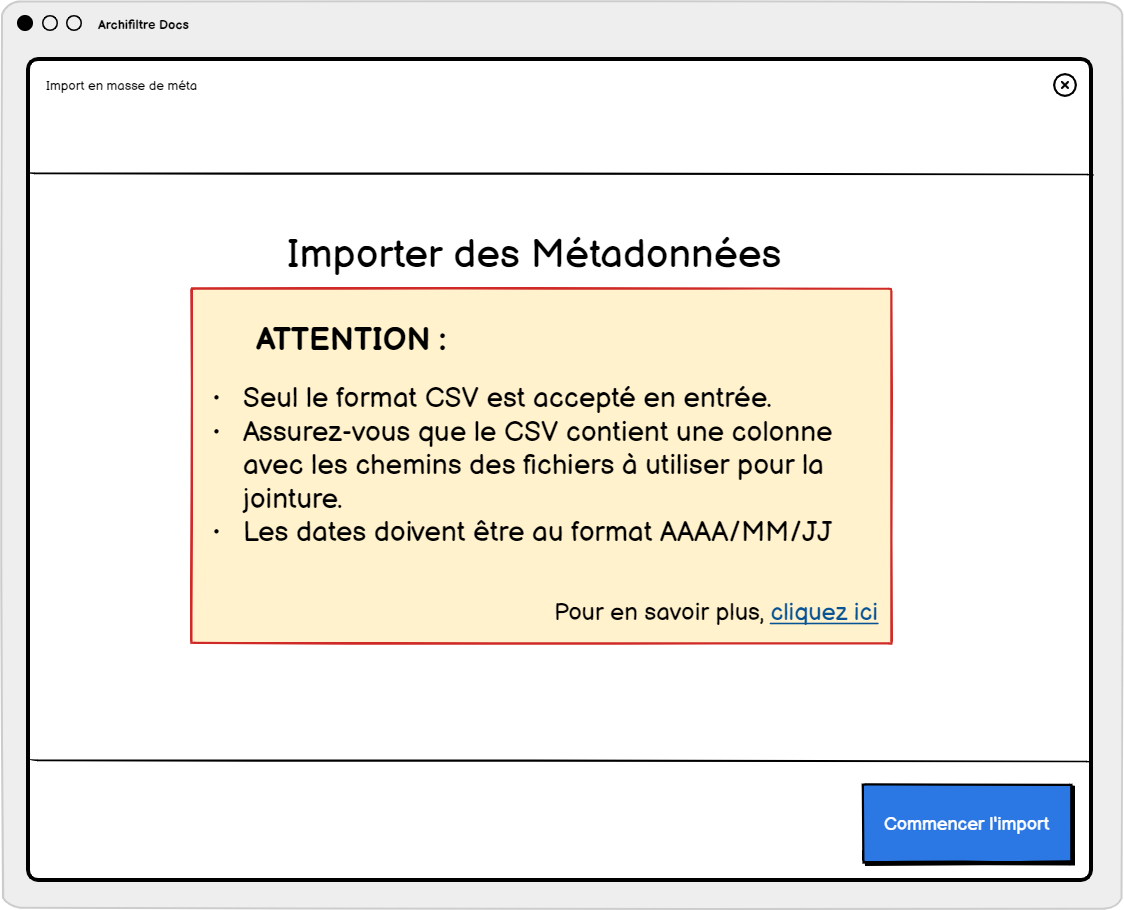
\includegraphics[width=\textwidth]{illustrations/figure21.png}
		\caption{Première version}
		\label{figure21}
	\end{minipage}
	\hfill %Met un espace entre les deux images.
	\begin{minipage}[b]{0.45\textwidth}
		\centering
		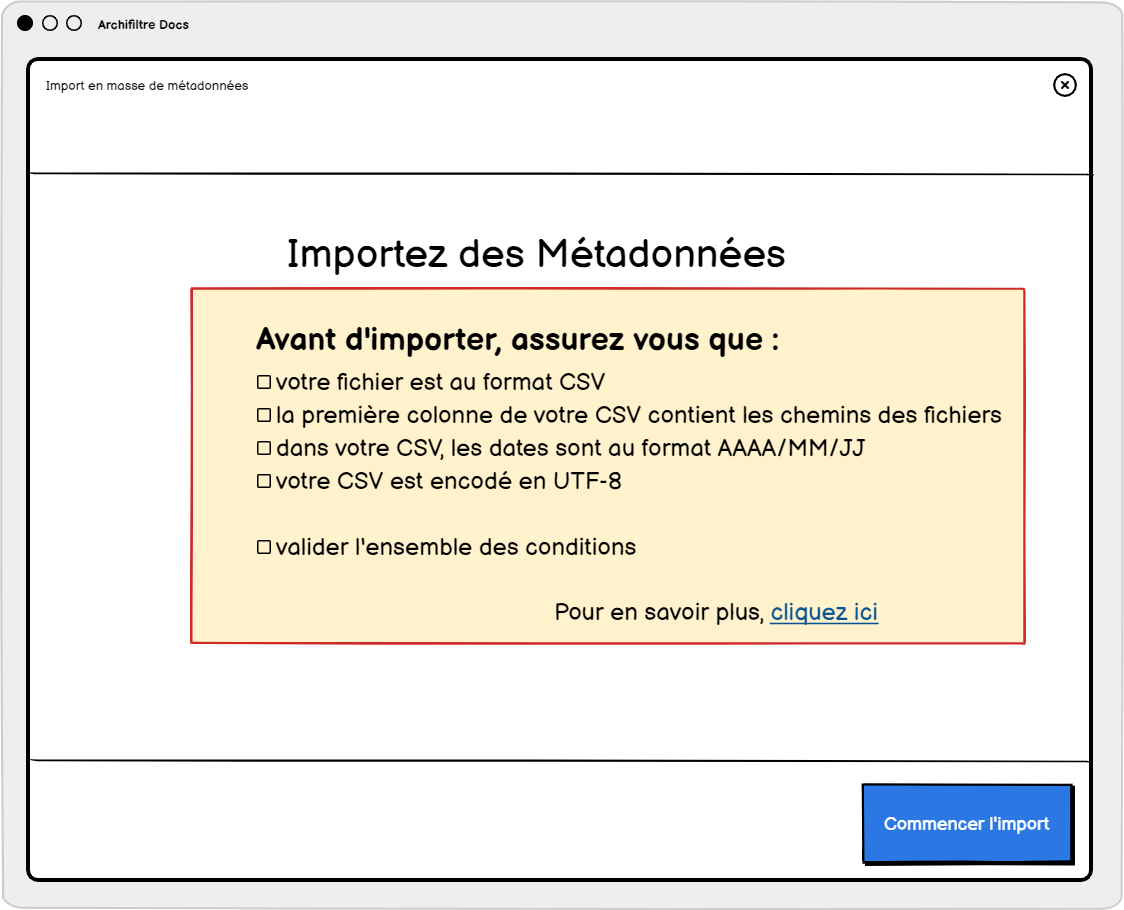
\includegraphics[width=\textwidth]{illustrations/figure22.png} 
		\caption{Version finale}
		\label{figure22}
	\end{minipage}
	\caption{Evolution des \textit{\gls{wireframe}s} de la fenêtre de vérification des contraintes à respecter avant import du CSV de métadonnées }
	\label{fig:sidebyside2}
\end{figure}


Pour présenter un cas plus détaillé d’évolution d’un \textit{\gls{wireframe}}, nous pouvons prendre l’exemple du \textit{\gls{wireframe}} le plus complexe à concevoir, celui permettant l’association de chaque métadonnée à une balise \gls{SEDA}.  La première version de ce \textit{\gls{wireframe}} s’inspirait de ce que propose ReSIP et proposait des escaliers de menus déroulants pour soit les métadonnées de gestion, soit les métadonnées de description. 

\clearpage

\insererImage{0.4}{illustrations/figure23.png}{Première version du \textit{\gls{wireframe}} d’association des métadonnées avec des balises \gls{SEDA}}{figure23}


Les tests utilisateurs et notamment celui d’Anne Lambert ont permis de faire ressortir les faiblesses de cette proposition, à savoir les difficultés de lisibilité pour les balises ayant un certain niveau de profondeur, quatre étant le nombre maximum. C’est par exemple le cas ci-dessus avec la balise <City>, sous-balise de <BirthPlace>, elle-même sous-balise de <Signer>, elle-même sous-balise de <Signature>, qui est une balise de <Content>, c'est-à-dire une métadonnée de description. Sa deuxième problématique réside dans le fait qu’une telle logique demande à l’utilisateur d’avoir préalablement une idée d’où aller chercher sa balise puisque les sous-balises n’apparaissent pas immédiatement. Anne Lambert nous a alors indiqué sa préférence pour une barre de recherche proposant de l’autocomplétion et associant le nom de la balise au chemin des balises dans laquelle elle se trouve comme le présente le \textit{\gls{wireframe}} suivant : 

\clearpage

\insererImage{0.4}{illustrations/figure24.png}{Deuxième version du \textit{\gls{wireframe}} d’association des métadonnées avec des balises \gls{SEDA}}{figure24}


A partir de cette idée, l’équipe a poursuivi les réflexions et a choisi de s’inspirer d'une interface, trouvée dans le cadre de nos recherches, qui semblait adaptée au besoin\footnote{Pour consulter l’interface : \href{https://baymard.com/ux-benchmark}{https://baymard.com/ux-benchmark}} et du double tableau présentant les sous-balises de <content> et de <management> présenté précédemment\footnote{Lien vers le double tableau en annexes \ref{annexeb} et \ref{annexec}} pour produire la version préférée des utilisateurs interrogés présentée ci-dessous. Ce \textit{\gls{wireframe}} propose pour chaque métadonnée à la fois une barre de recherche avec autocomplétion comme présenté dans le  \textit{\gls{wireframe}} précédent et à la fois une version améliorée des menus déroulants, présentant le nombre de sous-balise de chaque balise à tous les niveaux et reprenant les informations de définition de la balise, de répétabilité, de type et indiquant s’il s’agit d’une balise obligatoire comme cela a été mis en forme dans le double tableau des balises \gls{SEDA}. Par ailleurs, cette version propose deux options demandées par les utilisateurs : la possibilité de passer des noms de balises en français aux noms de balises en anglais ainsi que la possibilité de sauvegarder le balisage et ainsi de pouvoir l’effectuer de manière discontinue. 

\clearpage

\insererImage{0.35}{illustrations/figure25.png}{Version finale du \textit{\gls{wireframe}} d’association des métadonnées avec des balises \gls{SEDA}}{figure25}


\clearpage

Suivant cet exemple, un travail similaire, largement aidé des tests utilisateur, a été fait pour chaque \textit{\gls{wireframe}}. Cela a permis de fixer l’ensemble des \textit{\gls{wireframe}s} du processus de cette fonctionnalité d’import de métadonnées\footnote{Pour consulter le parcours de wireframes validés, voir annexe \ref{annexe9}}.

L’interface utilisateur du processus de la fonctionnalité d’import de métadonnées fixé, la prochaine étape consiste alors à commencer son développement. 

\chapter{Fermeture du deuxième diamant : développement et diffusion de la fonctionnalité}
\subsection{Spécifications fonctionnelles détaillées}

Afin de s’assurer que le développeur possède bien l’ensemble des informations nécessaires pour développer ce qui a été décidé par le précédent travail, le \textit{\gls{Product Manager}} et le \textit{\gls{Product Owner}} d’\gls{Archifiltre} écrivent les spécifications fonctionnelles détaillées. Ces dernières permettent de décrire en détail l’ensemble du comportement de chaque interface du processus. Il faut ainsi décrire par exemple l’effet produit par chaque bouton. Par ailleurs, l’équipe se sert du moment de sa rédaction également pour approfondir la réflexion sur les erreurs pouvant potentiellement se produire à chaque étape du processus. Elles sont listées dans les spécifications associées au message d’erreur à afficher pour chacune d'elles. Enfin, le développeur ayant suivi et parfois participé au travail effectué, la définition des spécifications se base également sur l’expertise technique qu’il a pu transmettre à l’équipe tout au long des choix faits lors des étapes précédentes permettant ainsi de prendre en compte les complexités techniques dans ces choix et d'éviter de mauvaises surprises plus tard comme par exemple des temps importants de développement supplémentaires. 


Traditionnellement, les spécifications prennent la forme d’une partie du cahier des charges et sont rédigées de manière linéaire, parfois appuyées d’images sans que cela ne soit systématique. Il en existe deux sortes : les spécifications fonctionnelles générales et les spécifications fonctionnelles détaillées. La première correspond dans la méthode \gls{Archifiltre} au \gls{PRD} et permet de faire l’étude générale du besoin alors que la deuxième permet de détailler la solution afin de guider le développement. \gls{Archifiltre} fait le choix d’une forme plus visuelle afin de rendre plus claires et instinctives ces spécifications fonctionnelles détaillées\footnote{Pour aller plus loin concernant l’amélioration des spécifications : \cite{cagan_revisiting_2006}}. Les \textit{\gls{wireframe}s} validés sont associés aux spécifications et chaque précision est liée à son emplacement sur le \textit{\gls{wireframe}} à l’aide de flèche comme ci-dessous : 

\insererImage{0.5}{illustrations/figure26.png}{Exemple de spécifications fonctionnelles détaillées associées au \gls{wireframe} de l'interface correspondante.\protect\footnotemark}{figure26}
\footnotetext{Zoom disponible en annexe \ref{annexe10}}

A partir de ces spécifications, le développeur va pouvoir organiser son travail et construire le produit attendu. Il est important de noter que ces dernières évolueront nécessairement, bien que le but lors de leur rédaction soit de les limiter autant que possible, en fonction des solutions techniques proposées par le développeur et des blocages qui peuvent apparaître. Des réunions à fréquence régulière sont donc organisées entre le développeur et le \textit{\gls{Product Manager}} afin de valider les choix techniques et leur impact sur ce qui a été défini dans les spécifications. 

\subsection{Adoption de la nouvelle fonctionnalité}


Lorsque les développements du \gls{MVP} seront terminés, un des enjeux essentiels de cette fonctionnalité devra alors être mené : son adoption par les services d’archives. Comme nous avons pu l’expliquer précédemment, la particularité de cette fonctionnalité est le fait que peu de services d’archives, et donc d’utilisateurs, se sont déjà saisis de la problématique à laquelle elle répond. Ainsi, il s’agit d’une fonctionnalité assez ambitieuse dont la volonté est de créer une méthodologie de traitement des systèmes d’information à archiver sans utiliser de connecteurs. Pour atteindre cet objectif, il est nécessaire de prévoir une stratégie de communication efficace afin de faciliter la prise en main de cette fonctionnalité relativement complexe. 


La première étape pour ce faire s’est mise en place lors des réflexions autour de la définition de l’interface utilisateur. En effet, un des enjeux était de rendre ce processus complexe le plus intuitif et clair possible. Pour ce faire, la notion de jointure a par exemple été rendue invisible pour l’utilisateur car les tests ont révélé une complexité, jugée finalement non nécessaire par l’équipe, à la compréhension de ce concept par les utilisateurs. Le choix final détaillé précédemment de l’interface d’association de balises \gls{SEDA} aux métadonnées qui propose la définition de chaque balise issue du dictionnaire du \gls{SEDA} 2.2 est également pensé afin de réduire la complexité du \gls{SEDA} qui repousse une partie des archivistes. Enfin, une documentation accompagnant la prise en main de la fonctionnalité par l’utilisateur va être proposée. Sa forme n’est pour le moment pas définie mais parmi les options envisagées se trouve la possibilité de fournir une arborescence test et un CSV de métadonnées associées ainsi qu’un pas à pas correspondant afin d’accompagner l’utilisateur dans sa première expérience de la fonctionnalité. Dans le but de créer la meilleure documentation possible, des entretiens utilisateurs pourront être organisés selon les principes de la méthode de travail générale de l’équipe \gls{Archifiltre}.  


La stratégie d’adoption de cette fonctionnalité imaginée par \gls{Archifiltre} consiste également à tester directement au sein du service des archives des Ministères sociaux cette solution et de documenter ce test. Ainsi, cette expérience pourra par la suite être partagée lors de présentations \gls{Archifiltre} et servir d’exemple. La méthode de traitement ainsi illustrée concrètement pourrait alors servir de base à l’appropriation de cette fonctionnalité par d’autres services d’archives. Par ailleurs, le fait d’échanger régulièrement avec les utilisateurs tout au long de ce développement a également permis d’impliquer des utilisateurs qui se feront potentiellement par la suite ambassadeurs de cette fonctionnalité au sein de leurs services.


Enfin, une communication par mail ainsi que sur les réseaux sociaux, notamment \textit{LinkedIn}, de manière plus classique sera également réalisée, s’intégrant dans le plan de communication général actuellement mis en place pour \gls{Archifiltre}. Cette communication permettra notamment dans un second temps d’obtenir des retours utilisateurs et de mesurer l’utilisation de cette fonctionnalité. Un plan de \textit{tracking}, qui sera mis en place lors du développement de la fonctionnalité, fournira également des statistiques complémentaires à ces retours et permettra d’évaluer sa conformité aux objectifs quantitatifs définis dans le \gls{PRD}. Ceux-ci seront décidés lors de la mise en place du \textit{tracking} mais se présentent comme des données chiffrées souhaitées sur une période donnée, comme par exemple le nombre d’utilisateurs ou le nombre de fichiers de métadonnées importés au premier mois. Cet ensemble permettra à l’équipe d’alimenter la \textit{\gls{story map}} et de continuer l’évolution et la correction de bugs de cette fonctionnalité dans de futures versions. 
\\

Ainsi, bien que le travail de cadrage de cette fonctionnalité soit terminé, il demeure deux parties essentielles de sa création à réaliser : le développement et la communication afin d’assurer son adoption puis d’en mesurer l’impact. Par ailleurs, l’ensemble de la méthodologie décrite dans cette troisième partie et présentée sur la base d’un exemple précis se fait ici l'exemple du déploiement de la stratégie innovante de gestion de projet d’\gls{Archifiltre}. 




	\chapter*{Conclusion}
	\addcontentsline{toc}{chapter}{Conclusion}
	
	Pour conclure, la chaîne de traitement des archives numériques au sein des Ministères est aujourd’hui relativement fixée et fonctionnelle en ce qui concerne les archives bureautiques. Cette méthodologie s’est en réalité créée à partir des normes et des outils qui la constituent. Au cœur de ces contraintes se trouve principalement le \gls{SEDA} et particulièrement ses versions limitées au sein de ces outils. Sa complexité et sa documentation assez pauvre pour l’instant constituent une difficulté parfois angoissante pour nombre d’archivistes et toujours difficile d’accès pour l’évolution des outils qui manipulent ce standard. Il est néanmoins à noter qu’un travail de refonte de la documentation est actuellement en cours au sein du SIAF pour la version 2.3 sortie fin juillet 2024 et devrait être disponible avant la fin de l’année 2024. 
	
	
	Afin de faire évoluer l’outil \gls{Archifiltre}, il était donc indispensable de pleinement comprendre aussi bien le \gls{SEDA} que la chaîne de traitement définie et ses outils. En effet, l’archivage numérique reste aujourd’hui complexe et pour réussir une nouvelle fonctionnalité, il est primordial d’une part qu’elle respecte les contraintes techniques imposées et d’autre part qu’elle se présente comme complétant logiquement cette chaîne à laquelle les professionnels sont déjà habitués. En effet, son adoption serait bien plus difficile si elle semblait demander de ré-apprendre tous les savoirs du traitement des archives numériques pour l’utiliser. Par ailleurs, la fonctionnalité présentée dans ce travail doit également s’adapter techniquement à l’objet qu’il propose de traiter afin d’en faciliter son archivage : les systèmes d’information. Ces objets dont la forme diffère de l’un à l’autre présentent aujourd’hui une difficulté particulière dans leur archivage, ce que l'exposition des exemples de cas d’usage d’archivage de SI rencontrés par le service des archives des Ministères sociaux permet de mettre en lumière.
	
	
	Ainsi, l’équipe \gls{Archifiltre} a déployé pour réussir l’évolution de leur outil avec cette nouvelle fonctionnalité une méthodologie innovante basée sur l’approche produit et les méthodes agiles. L’adaptabilité de cette méthode et l’importance donnée aux retours utilisateurs tout au long du développement, ainsi que la rigueur qu’impose l’utilisation du \gls{PRD} qui guide l’ensemble des réflexions et empêche de s’éloigner du sujet, ont permis de faire évoluer \gls{Archifiltre} tout en vérifiant continuellement sa cohérence avec l’environnement technique auquel il participe. Par ailleurs, le principe de proposer d’abord un \gls{MVP} et de le faire évoluer ensuite au fil des nouvelles versions de l'application permet de réajuster l’accord au cadre technique défini en cas de problème mais aussi de s’adapter aux évolutions de ce cadre.
	
	
	Enfin, bien que ce travail expose légitimement l’importance de l’évolution des outils afin de répondre aux besoins techniques de l’archivage électronique d’objets toujours plus complexes, il serait intéressant de remettre en perspective la course à l’innovation et à l’amélioration dans laquelle s’inscrit cette démarche. Dans son article \enquote{Technologies de l’information : rupture ou continuité ?}\footcite{chabin_technologies_2017} (2017), Marie Anne Chabin fait notamment la constatation de l’ \enquote{accélération du remplacement des technologies récentes de gestion de l’information par des technologies encore plus récentes}. En effet, l’ère du numérique accélère non seulement la production documentaire mais également l’évolution et l’obsolescence des outils destinés à son traitement et à son archivage. Dans un milieu où le but principal est d’atteindre la pérennisation de l’information, il est légitime de se demander si cette course actuelle au développement des logiciels est toujours pertinente. La création d’Archifiltre et le développement de la fonctionnalité décrite tout au long de ce travail ont une utilité indéniable aujourd’hui pour répondre aux problématiques rencontrées par les archivistes numériques. Néanmoins, il est important de se demander à quel stade peut-on considérer un outil comme abouti ? Comment faire en sorte d’en pérenniser l’usage plutôt que de voir les professionnels contraints de changer d’outil pour s’adapter aux exigences de leur métier ? Finalement, à mesure que la chaîne de traitement se fixe, sera-t-il possible d’atteindre une stabilité dans les outils ou sommes-nous contraints à continuer la course à leur l’amélioration ? Gagnera-t-on un jour cette course ? 
	
	
	\enquote{L’enjeu n’est-il pas aussi, au-delà des technologies, d’analyser les permanences et les révolutions fonctionnelles et sociétales qu’elles induisent, afin de permettre aux managers et à leurs collaborateurs de MIEUX utiliser ces technologies et pas seulement de les utiliser PLUS ?} - MA Chabin\footcite{chabin_technologies_2017}
	
\newpage{\pagestyle{empty}\cleardoublepage}
	






%%%%%%%%%%%%%%%%%%

\appendix %Des appendices: tables figures, annexes, table des matière.
	
	\part*{Annexes}	
	\addcontentsline{toc}{part}{Annexes}
	
	\chapter[Frise chronologique Archifiltre]{Frise chronologique de la création d’Archifiltre réalisée par Manon Saget-Lethias.}
	\begin{landscape}
		\begin{figure}[h]
			\centering
			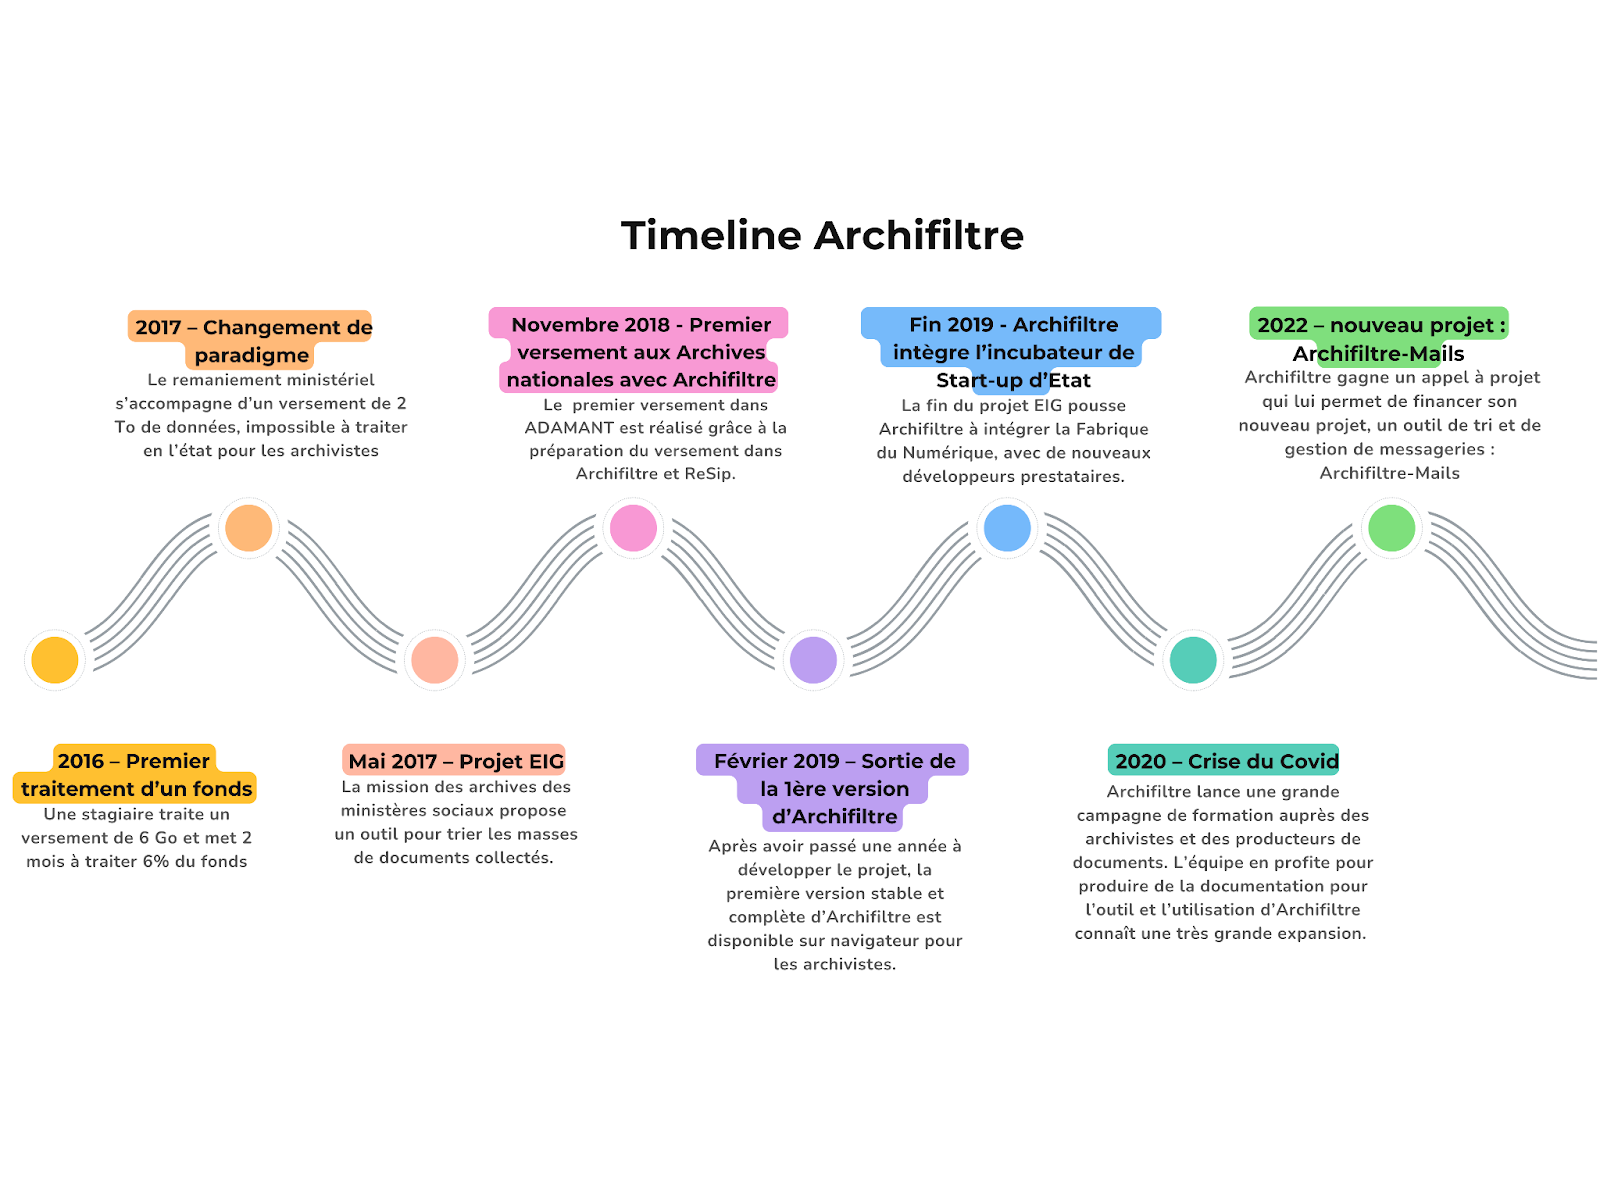
\includegraphics[scale=0.45]{annexes/annexe1.png}
			\label{annexe1}
		\end{figure}
	\end{landscape}
	
	\chapter[Balises métadonnées de description]{Tableau des balises des métadonnées de description d'une Unité d'archive en SEDA 2.2}

	\begin{landscape}
		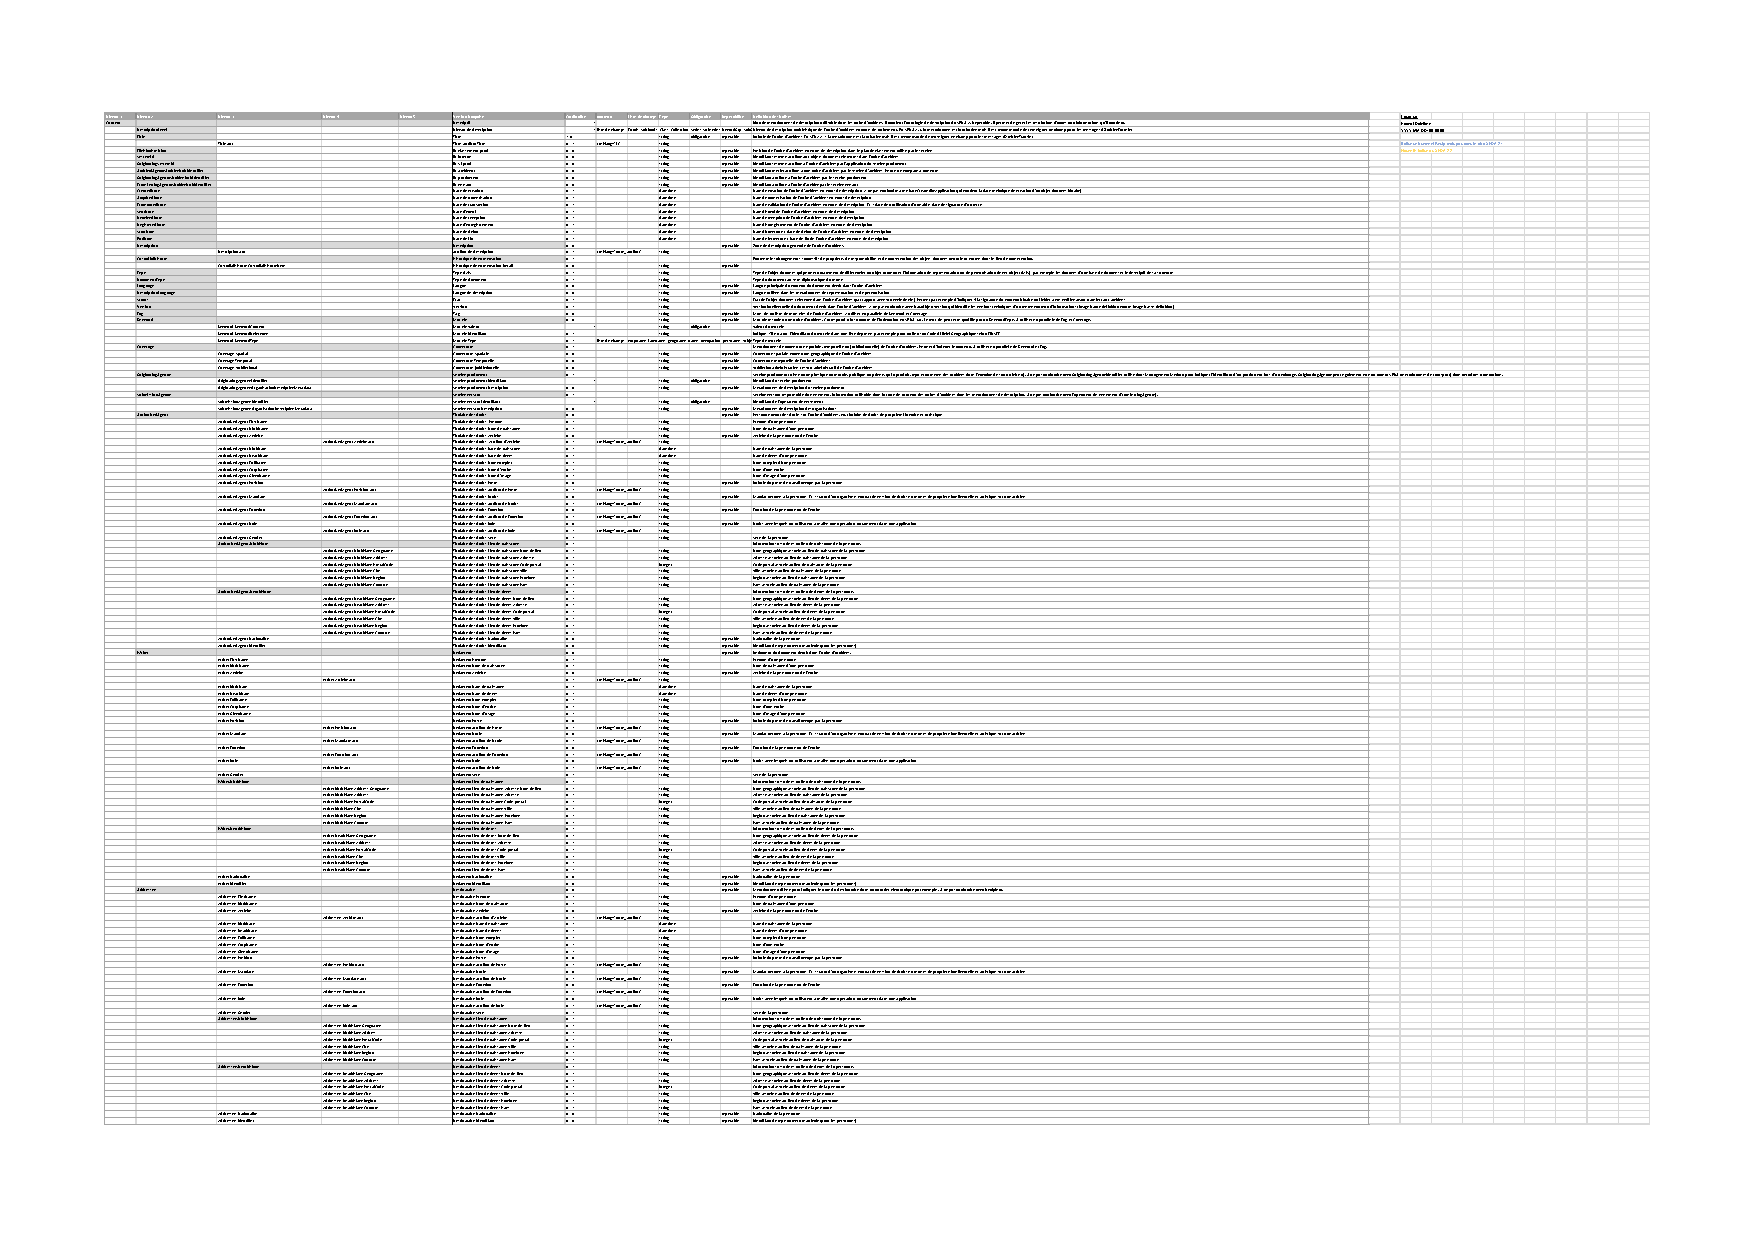
\includepdf[pages=-, scale=1,landscape=true]{annexes/Balisage SEDA-Resip export de métadonnées - Métadonnées de description.pdf}
	\end{landscape}
	\label{annexeb}
	
	\chapter[Balises métadonnées de gestion]{Tableau des balises des métadonnées de gestion d'une Unité d'archive en SEDA 2.2}
	\begin{landscape}
		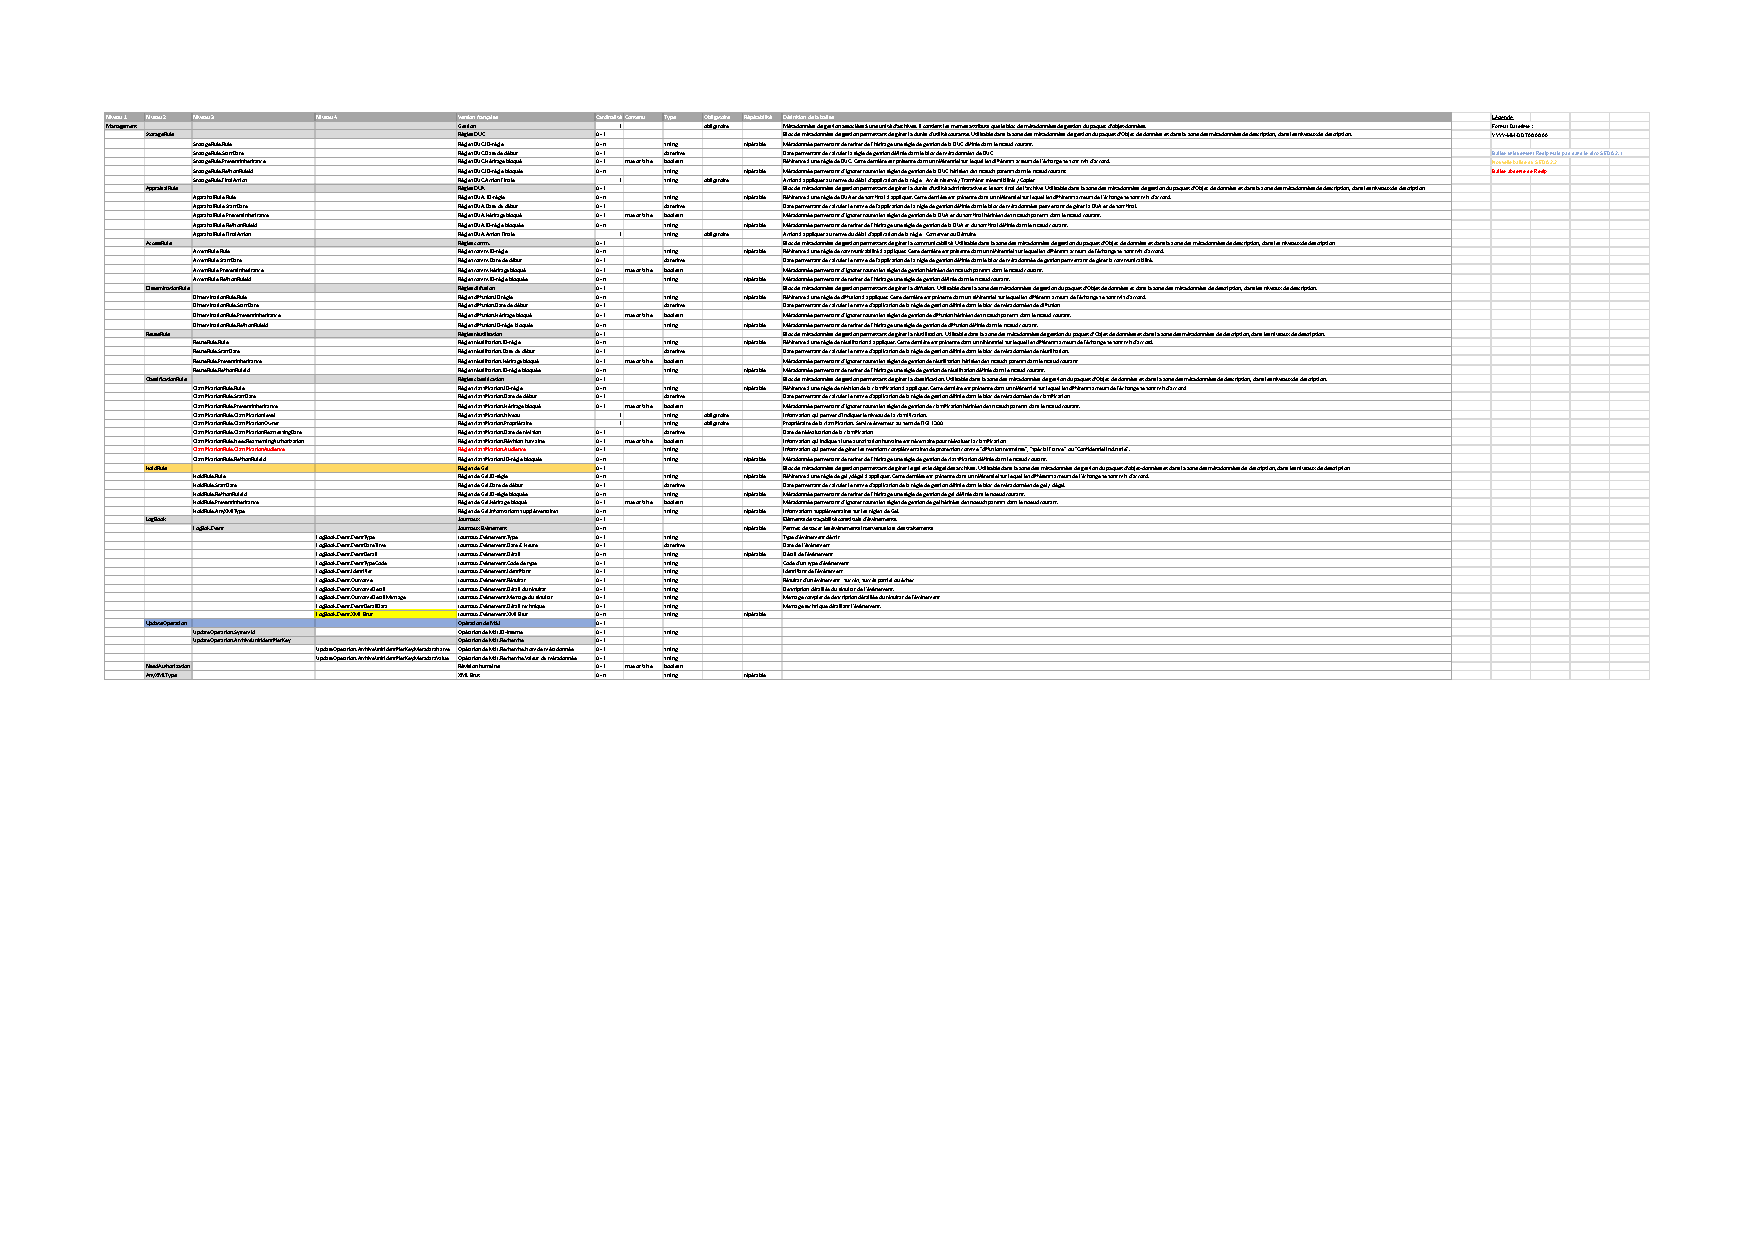
\includepdf[pages=-, scale=1,landscape=true]{annexes/Balisage SEDA-Resip export de métadonnées - Métadonnées de gestion.pdf}
	\end{landscape}
	\label{annexec}

	\chapter[Grille étude CYCLAD]{Grille vierge pour réaliser une étude CYCLAD crée par le bureau des archives du Ministère de l'Agriculture}
	\begin{landscape}
		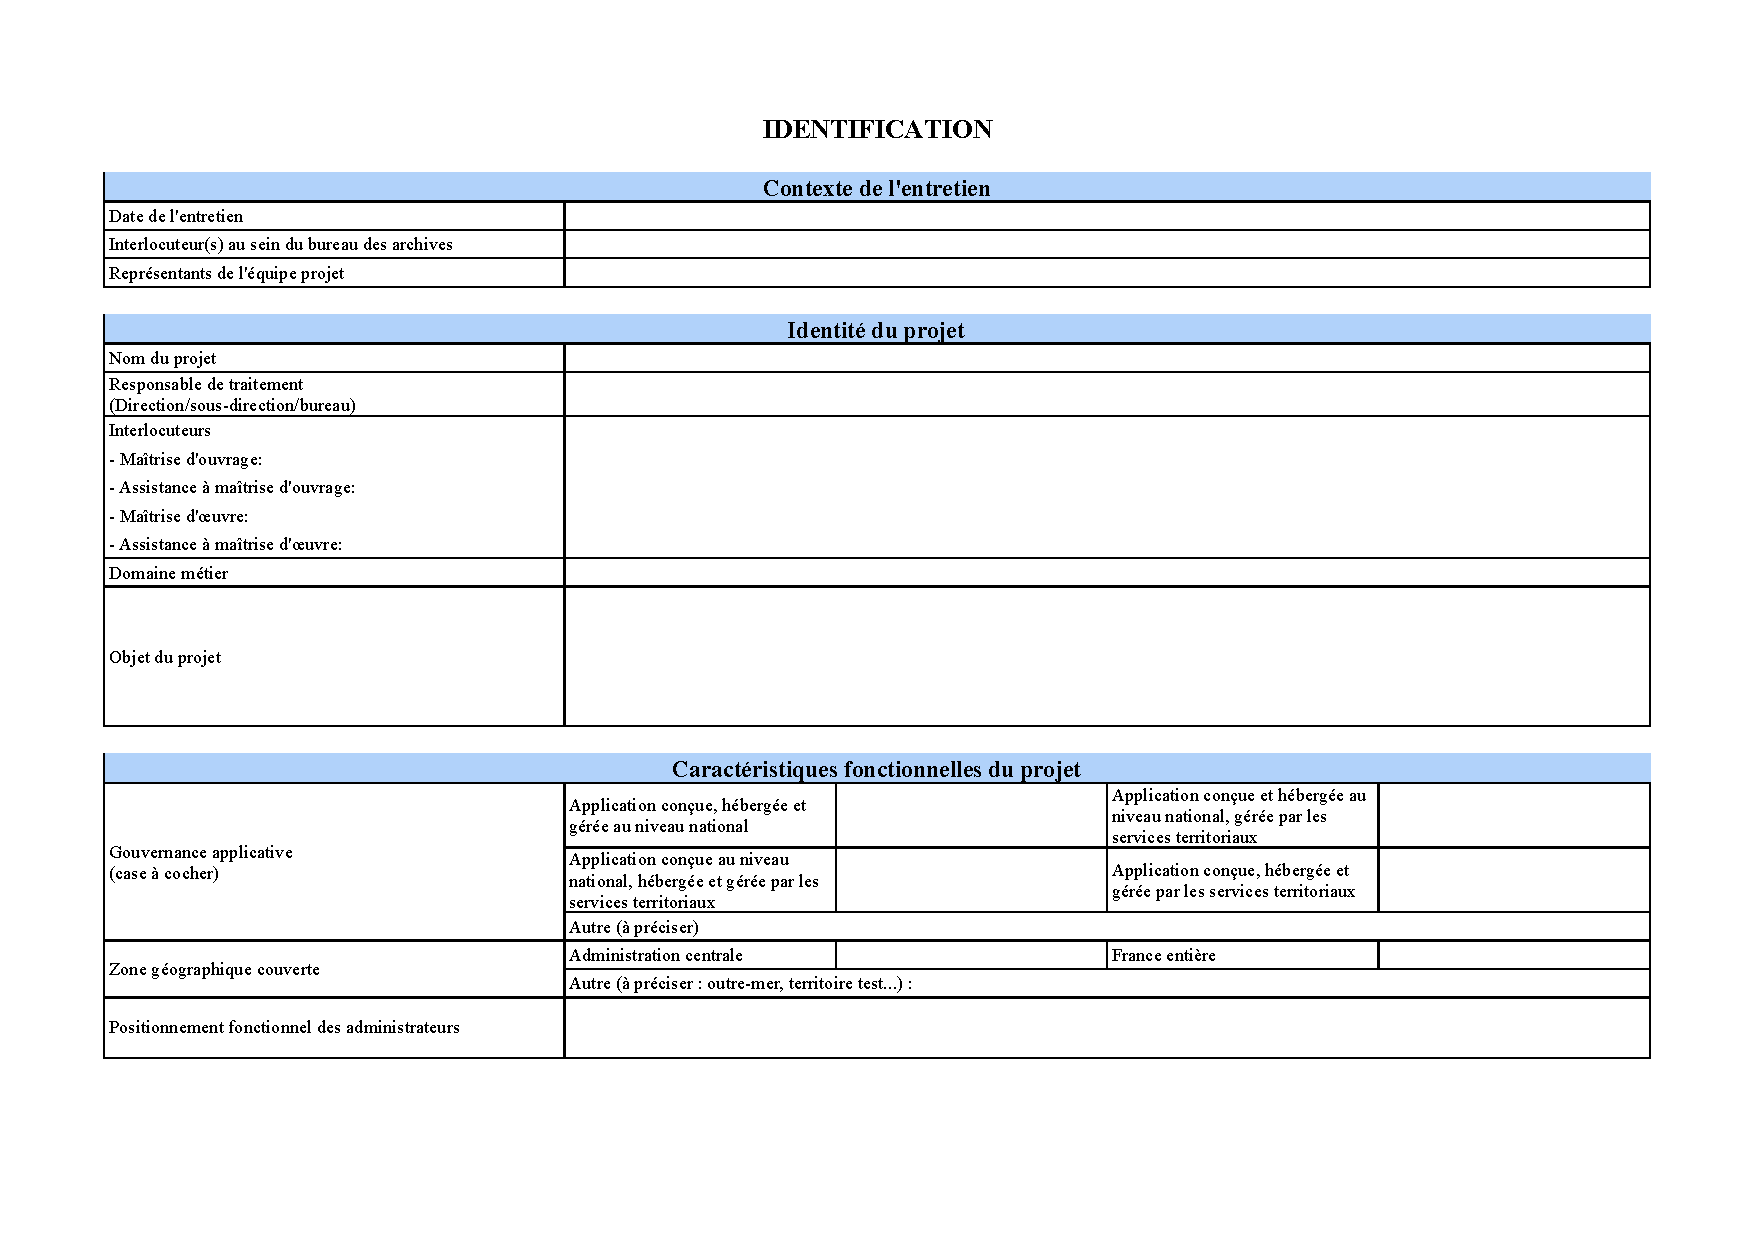
\includepdf[pages=-, scale=1,landscape=true]{annexes/grilleCyclad.pdf}
	\end{landscape}
	\label{annexed}
	
	\chapter[PRD vierge]{Squelette vierge d'un PRD}
	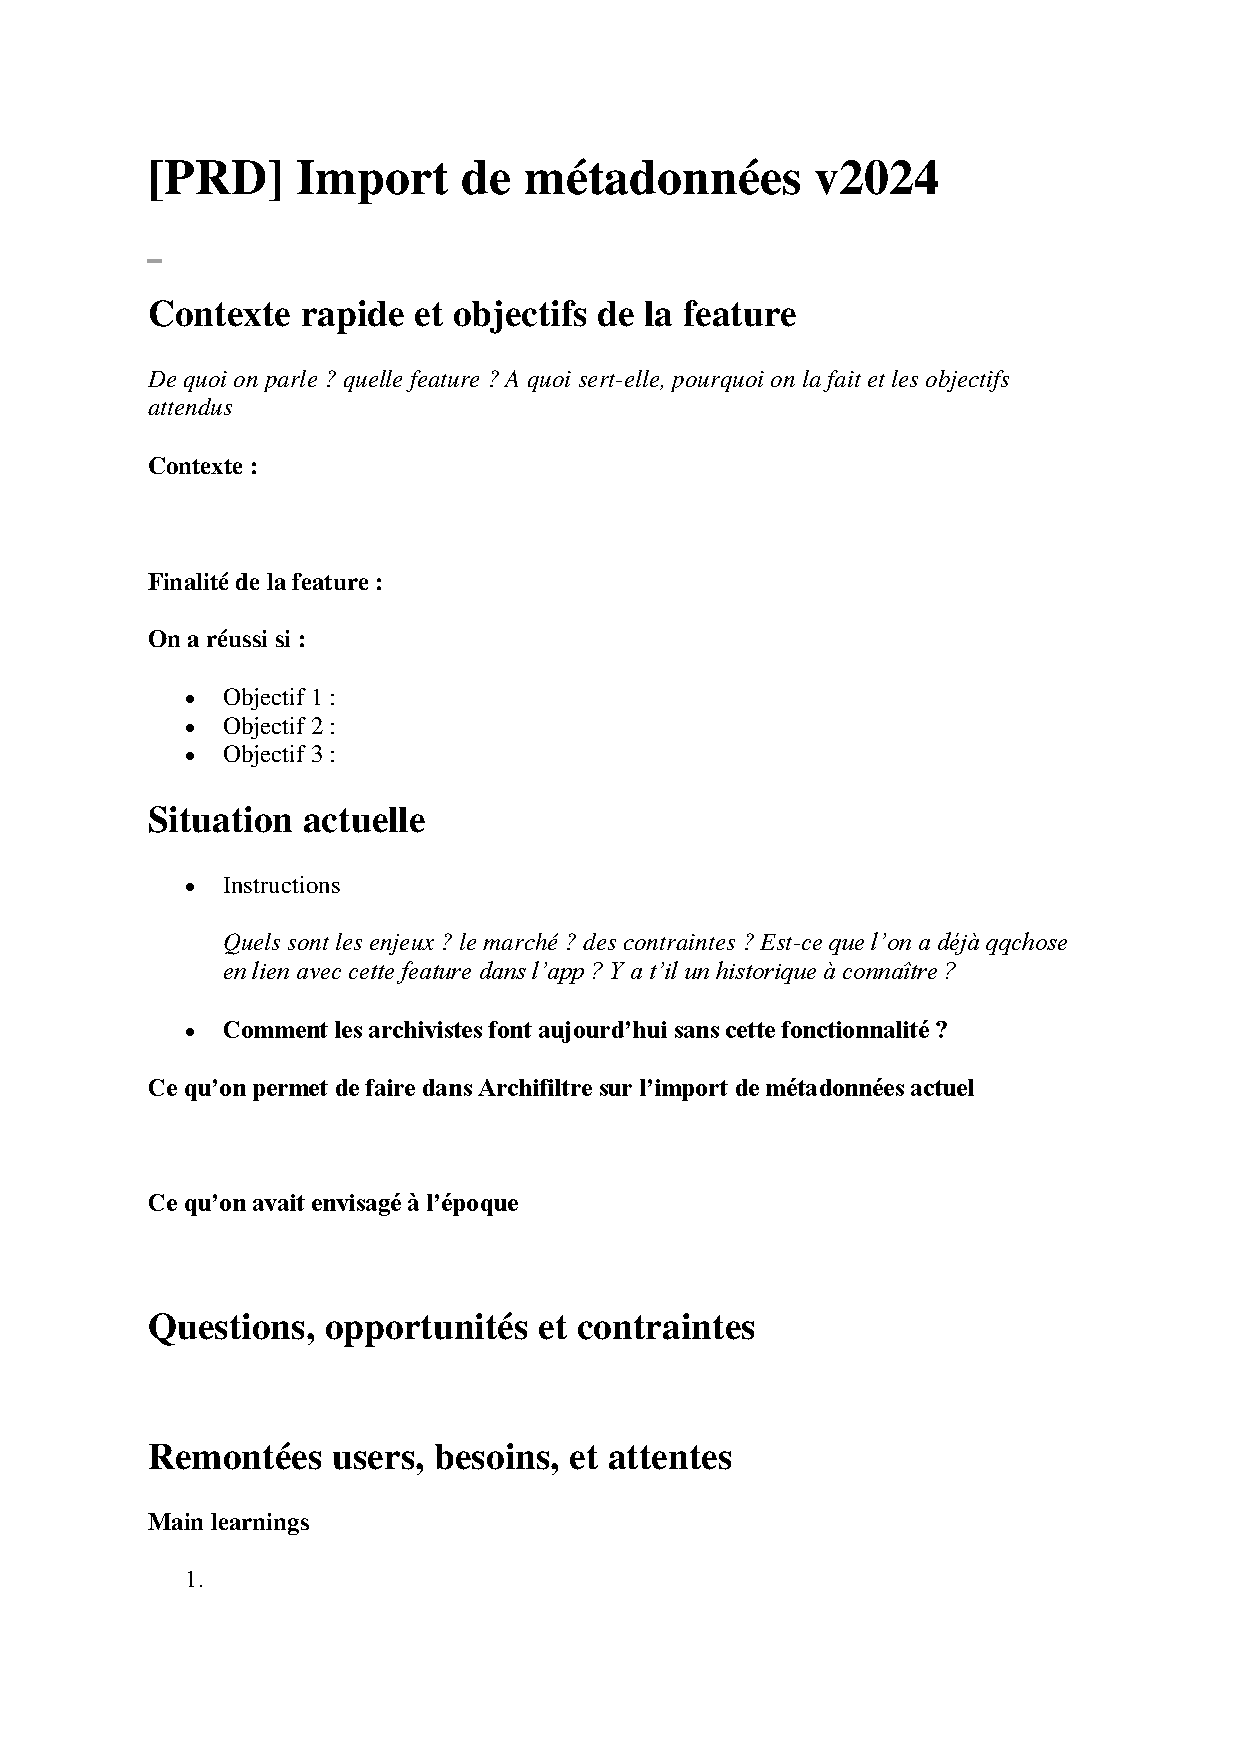
\includepdf[pages=-, scale=1]{annexes/PRDvierge.pdf}
	\label{annexee}
	
	\chapter[Mode projet et mode produit]{Tableau comparatif de l’approche projet comparée à l’approche produit par beta.gouv\footcite[pp.45-46]{betagouv_guide_2024}}
	\begin{figure}[h]
		\centering
		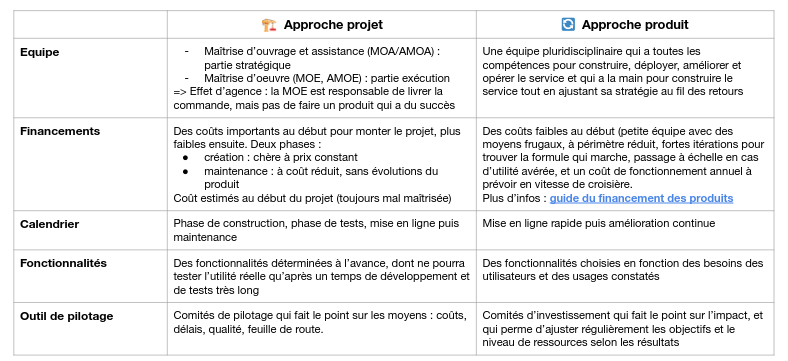
\includegraphics[scale=0.45]{annexes/annexe4.1.png}
		\label{annexe4.1}
	\end{figure}
	\begin{figure}[h]
		\centering
		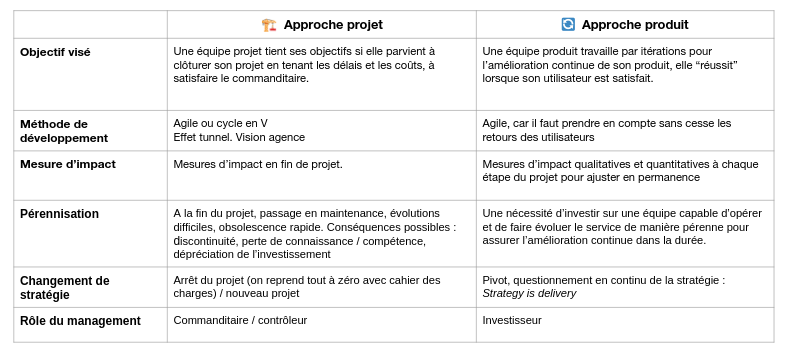
\includegraphics[scale=0.45]{annexes/annexe4.2.png}
		\label{annexe4.2}
	\end{figure}

	\chapter[Schéma lean startup]{Schéma des principes du \textit{lean startup} par beta.gouv\footcite[p.18]{betagouv_guide_2024}}
	\begin{figure}[h]
		\centering
		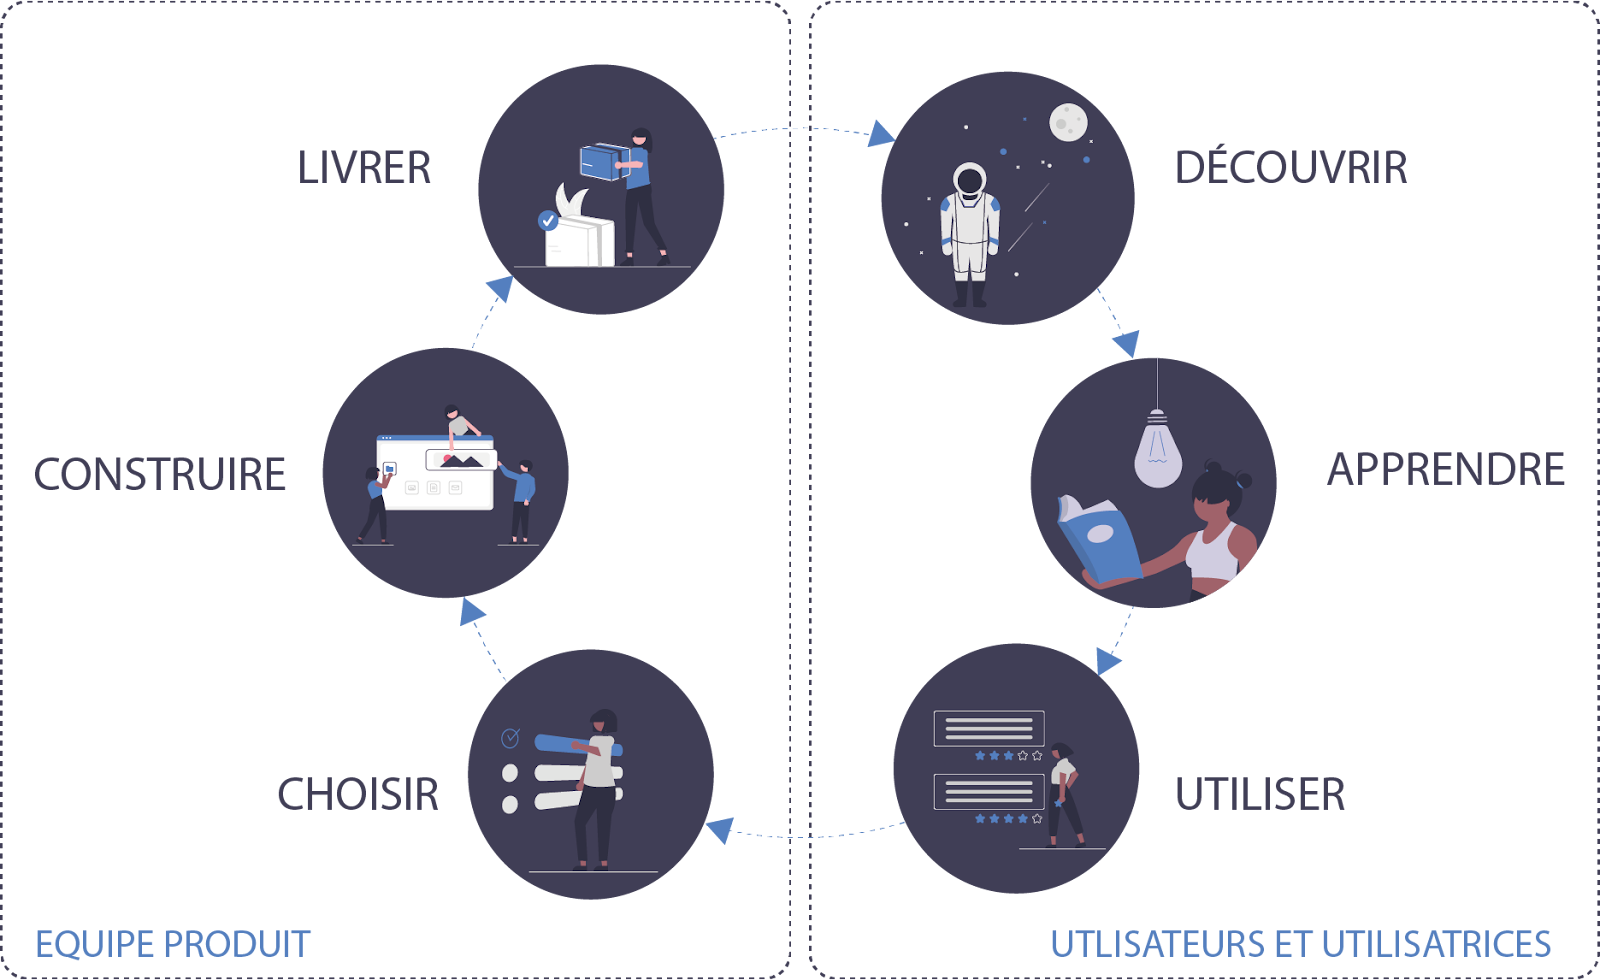
\includegraphics[scale=0.3]{annexes/annexe5.png}
		\label{annexe5}
	\end{figure}

	\chapter[Zooms diagramme d'utilisation]{Zooms sur le diagramme d'utilisation de la fonctionnalité import de métadonnées dans \gls{Archifiltre}
	}

	\begin{figure}[h]
		\centering
		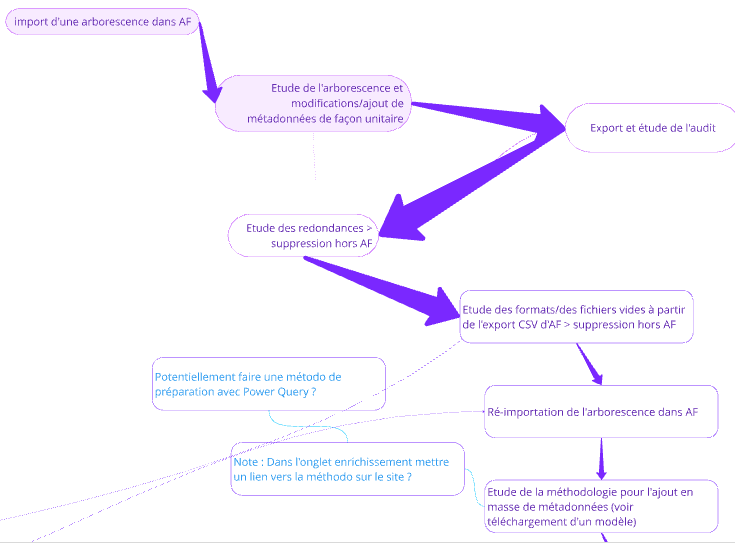
\includegraphics[scale=0.5]{annexes/annexe6.png}
		\caption{Premier zoom}
		\label{annexe6}
	\end{figure}

	\begin{figure}[h]
		\centering
		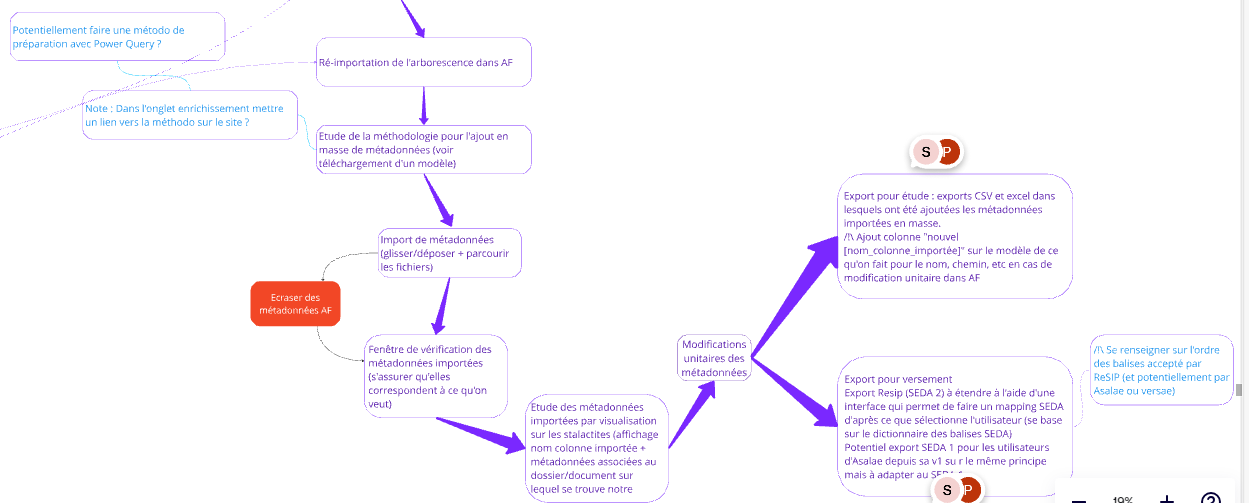
\includegraphics[scale=0.4]{annexes/annexe6.2.png}
		\caption{Deuxième zoom}
		\label{annexe6.2}
	\end{figure}
	
	\chapter[Import ReSIP]{Exemple de structure d'un fichier accepté en import dans ReSIP} 
	\begin{figure}[h]
		\centering
		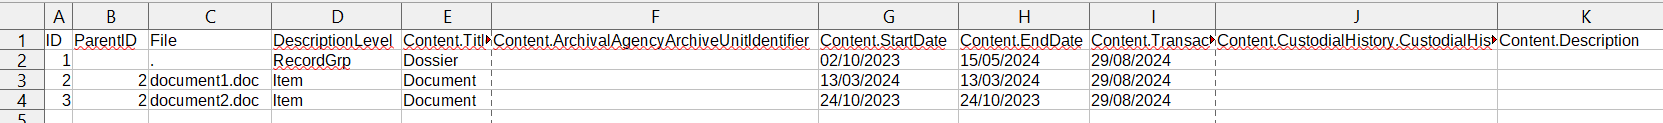
\includegraphics[scale=0.6]{annexes/annexe7.png}
		\label{annexe7}
	\end{figure}
	
	\chapter[Zooms story map]{Zooms sur la \textit{user \gls{story map}} de la fonctionnalité import de métadonnées}

Premier zoom :
	\begin{figure}[h]
		\centering
		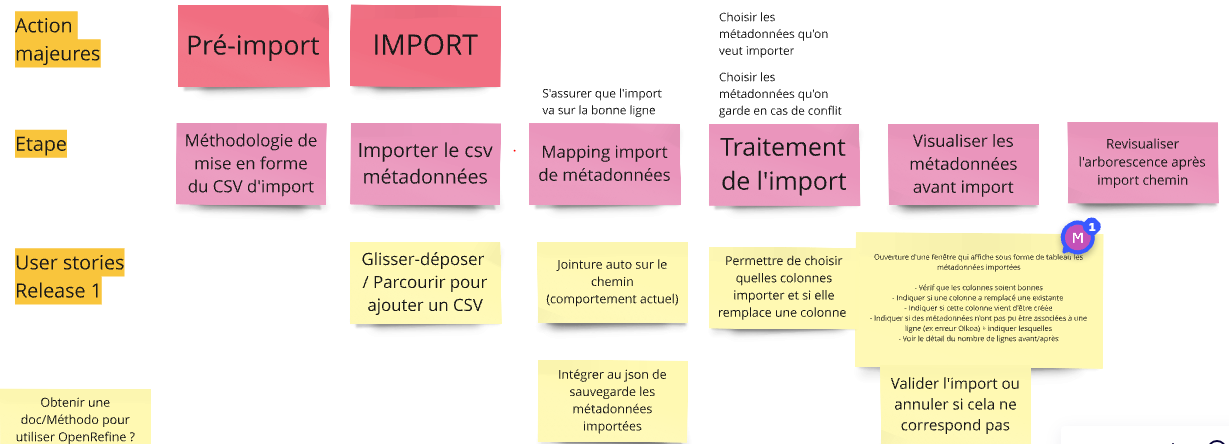
\includegraphics[scale=0.4]{annexes/annexe8.1.png}
		\caption{Premier zoom}
		\label{annexe8.1}
	\end{figure}
Deuxième zoom :
	\begin{figure}[h]
		\centering
		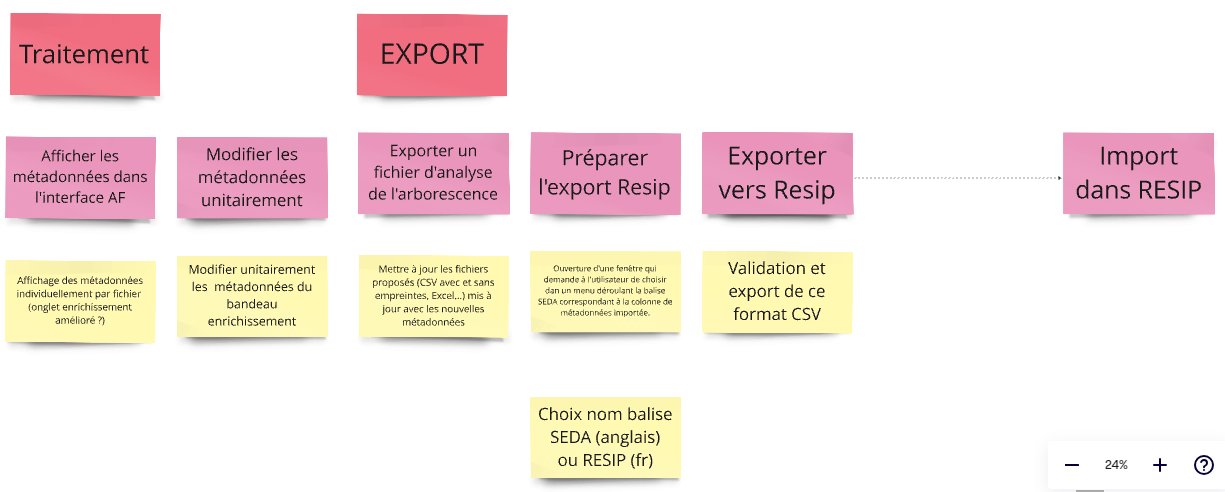
\includegraphics[scale=0.4]{annexes/annexe8.2.png}
		\caption{Deuxième zoom}
		\label{annexe8.2}
	\end{figure}

	\chapter[Wireframes validés]{Wireframes du parcours utilisateur validés}
	\includepdf[pages=-, scale=1,landscape=true]{annexes/Chemin wireframes validé.pdf}
	\label{annexe9}

	\chapter[Zoom spécifications fonctionnelles]{Zoom sur l'exemple de spécifications fonctionnelles détaillées associées au \gls{wireframe} de l'interface correspondante.}
	\begin{figure}[h]
		\centering
		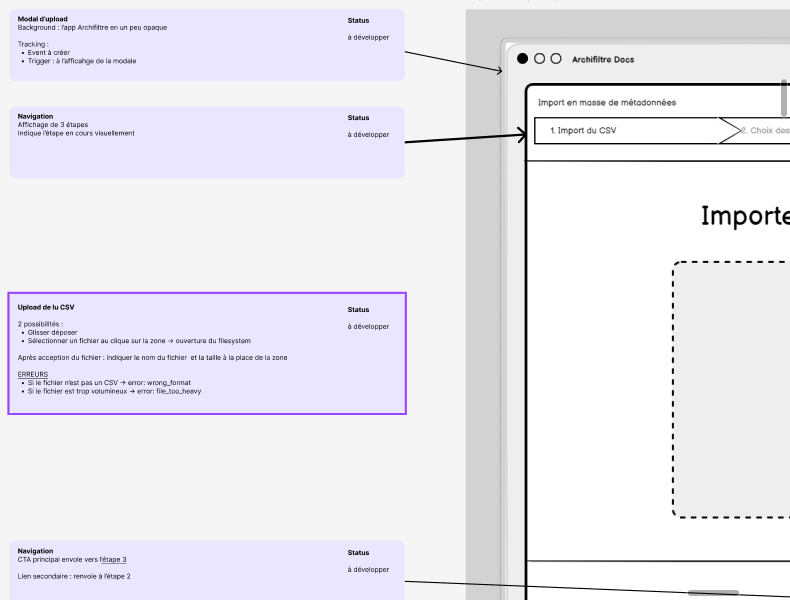
\includegraphics[scale=0.55]{annexes/annexe9.png}
		\label{annexe10}
	\end{figure}

\newpage{\pagestyle{empty}\cleardoublepage}

%%%%%%%%%%%%%%%%%%

\backmatter % glossaire, table des figures, table des matières. 

\printglossaries
\textit{Ce glossaire a été rédigé avec l'aide de Chat GPT.}

\listoffigures
\tableofcontents
\end{document}
